\documentclass[]{article}
\usepackage{lmodern}
\usepackage{amssymb,amsmath}
\usepackage{ifxetex,ifluatex}
\usepackage{fixltx2e} % provides \textsubscript
\ifnum 0\ifxetex 1\fi\ifluatex 1\fi=0 % if pdftex
  \usepackage[T1]{fontenc}
  \usepackage[utf8]{inputenc}
\else % if luatex or xelatex
  \ifxetex
    \usepackage{mathspec}
  \else
    \usepackage{fontspec}
  \fi
  \defaultfontfeatures{Ligatures=TeX,Scale=MatchLowercase}
\fi
% use upquote if available, for straight quotes in verbatim environments
\IfFileExists{upquote.sty}{\usepackage{upquote}}{}
% use microtype if available
\IfFileExists{microtype.sty}{%
\usepackage{microtype}
\UseMicrotypeSet[protrusion]{basicmath} % disable protrusion for tt fonts
}{}
\usepackage[margin=1in]{geometry}
\usepackage{hyperref}
\hypersetup{unicode=true,
            pdftitle={MovieLens Recommender System Capstone Project - Report},
            pdfauthor={Alessandro Corradini - Harvard Data Science Professional},
            pdfborder={0 0 0},
            breaklinks=true}
\urlstyle{same}  % don't use monospace font for urls
\usepackage{color}
\usepackage{fancyvrb}
\newcommand{\VerbBar}{|}
\newcommand{\VERB}{\Verb[commandchars=\\\{\}]}
\DefineVerbatimEnvironment{Highlighting}{Verbatim}{commandchars=\\\{\}}
% Add ',fontsize=\small' for more characters per line
\newenvironment{Shaded}{}{}
\newcommand{\AlertTok}[1]{\textcolor[rgb]{1.00,0.00,0.00}{\textbf{#1}}}
\newcommand{\AnnotationTok}[1]{\textcolor[rgb]{0.38,0.63,0.69}{\textbf{\textit{#1}}}}
\newcommand{\AttributeTok}[1]{\textcolor[rgb]{0.49,0.56,0.16}{#1}}
\newcommand{\BaseNTok}[1]{\textcolor[rgb]{0.25,0.63,0.44}{#1}}
\newcommand{\BuiltInTok}[1]{#1}
\newcommand{\CharTok}[1]{\textcolor[rgb]{0.25,0.44,0.63}{#1}}
\newcommand{\CommentTok}[1]{\textcolor[rgb]{0.38,0.63,0.69}{\textit{#1}}}
\newcommand{\CommentVarTok}[1]{\textcolor[rgb]{0.38,0.63,0.69}{\textbf{\textit{#1}}}}
\newcommand{\ConstantTok}[1]{\textcolor[rgb]{0.53,0.00,0.00}{#1}}
\newcommand{\ControlFlowTok}[1]{\textcolor[rgb]{0.00,0.44,0.13}{\textbf{#1}}}
\newcommand{\DataTypeTok}[1]{\textcolor[rgb]{0.56,0.13,0.00}{#1}}
\newcommand{\DecValTok}[1]{\textcolor[rgb]{0.25,0.63,0.44}{#1}}
\newcommand{\DocumentationTok}[1]{\textcolor[rgb]{0.73,0.13,0.13}{\textit{#1}}}
\newcommand{\ErrorTok}[1]{\textcolor[rgb]{1.00,0.00,0.00}{\textbf{#1}}}
\newcommand{\ExtensionTok}[1]{#1}
\newcommand{\FloatTok}[1]{\textcolor[rgb]{0.25,0.63,0.44}{#1}}
\newcommand{\FunctionTok}[1]{\textcolor[rgb]{0.02,0.16,0.49}{#1}}
\newcommand{\ImportTok}[1]{#1}
\newcommand{\InformationTok}[1]{\textcolor[rgb]{0.38,0.63,0.69}{\textbf{\textit{#1}}}}
\newcommand{\KeywordTok}[1]{\textcolor[rgb]{0.00,0.44,0.13}{\textbf{#1}}}
\newcommand{\NormalTok}[1]{#1}
\newcommand{\OperatorTok}[1]{\textcolor[rgb]{0.40,0.40,0.40}{#1}}
\newcommand{\OtherTok}[1]{\textcolor[rgb]{0.00,0.44,0.13}{#1}}
\newcommand{\PreprocessorTok}[1]{\textcolor[rgb]{0.74,0.48,0.00}{#1}}
\newcommand{\RegionMarkerTok}[1]{#1}
\newcommand{\SpecialCharTok}[1]{\textcolor[rgb]{0.25,0.44,0.63}{#1}}
\newcommand{\SpecialStringTok}[1]{\textcolor[rgb]{0.73,0.40,0.53}{#1}}
\newcommand{\StringTok}[1]{\textcolor[rgb]{0.25,0.44,0.63}{#1}}
\newcommand{\VariableTok}[1]{\textcolor[rgb]{0.10,0.09,0.49}{#1}}
\newcommand{\VerbatimStringTok}[1]{\textcolor[rgb]{0.25,0.44,0.63}{#1}}
\newcommand{\WarningTok}[1]{\textcolor[rgb]{0.38,0.63,0.69}{\textbf{\textit{#1}}}}
\usepackage{graphicx,grffile}
\makeatletter
\def\maxwidth{\ifdim\Gin@nat@width>\linewidth\linewidth\else\Gin@nat@width\fi}
\def\maxheight{\ifdim\Gin@nat@height>\textheight\textheight\else\Gin@nat@height\fi}
\makeatother
% Scale images if necessary, so that they will not overflow the page
% margins by default, and it is still possible to overwrite the defaults
% using explicit options in \includegraphics[width, height, ...]{}
\setkeys{Gin}{width=\maxwidth,height=\maxheight,keepaspectratio}
\IfFileExists{parskip.sty}{%
\usepackage{parskip}
}{% else
\setlength{\parindent}{0pt}
\setlength{\parskip}{6pt plus 2pt minus 1pt}
}
\setlength{\emergencystretch}{3em}  % prevent overfull lines
\providecommand{\tightlist}{%
  \setlength{\itemsep}{0pt}\setlength{\parskip}{0pt}}
\setcounter{secnumdepth}{5}
% Redefines (sub)paragraphs to behave more like sections
\ifx\paragraph\undefined\else
\let\oldparagraph\paragraph
\renewcommand{\paragraph}[1]{\oldparagraph{#1}\mbox{}}
\fi
\ifx\subparagraph\undefined\else
\let\oldsubparagraph\subparagraph
\renewcommand{\subparagraph}[1]{\oldsubparagraph{#1}\mbox{}}
\fi

%%% Use protect on footnotes to avoid problems with footnotes in titles
\let\rmarkdownfootnote\footnote%
\def\footnote{\protect\rmarkdownfootnote}

%%% Change title format to be more compact
\usepackage{titling}

% Create subtitle command for use in maketitle
\providecommand{\subtitle}[1]{
  \posttitle{
    \begin{center}\large#1\end{center}
    }
}

\setlength{\droptitle}{-2em}

  \title{MovieLens Recommender System Capstone Project - Report}
    \pretitle{\vspace{\droptitle}\centering\huge}
  \posttitle{\par}
    \author{Alessandro Corradini - Harvard Data Science Professional}
    \preauthor{\centering\large\emph}
  \postauthor{\par}
      \predate{\centering\large\emph}
  \postdate{\par}
    \date{5 May, 2019}


\begin{document}
\maketitle

{
\setcounter{tocdepth}{2}
\tableofcontents
}
\newpage

\hypertarget{executive-summary}{%
\section{Executive Summary}\label{executive-summary}}

The purpose for this project is creating a recommender system using
MovieLens dataset.

The version of movielens dataset used for this final assignment contains
approximately 10 Milions of movies ratings, divided in 9 Milions for
training and one Milion for validation. It is a small subset of a much
larger (and famous) dataset with several millions of ratings. Into the
training dataset there are approximately 70.000 users and 11.000
different movies divided in 20 genres such as Action, Adventure, Horror,
Drama and Thriller.

After a initial data exploration, the recommender systems builted on
this dataset are evaluated and choosen based on the RMSE - Root Mean
Squared Error that should be at least lower than 0.87750.

\[\mbox{RMSE} = \sqrt{\frac{1}{n}\sum_{t=1}^{n}e_t^2}\]

\hypertarget{exploratory-data-analysis}{%
\section{Exploratory Data Analysis}\label{exploratory-data-analysis}}

\hypertarget{inital-data-exploration}{%
\subsection{Inital data Exploration}\label{inital-data-exploration}}

The 10 Millions dataset is divided into two dataset: \texttt{edx} for
training purpose and \texttt{validation} for the validation phase.

The \texttt{edx} dataset contains approximately 9 Millions of rows with
70.000 different users and 11.000 movies with rating score between 0.5
and 5. There is no missing values (0 or NA).

\textbf{edx dataset}

\begin{table}[H]
\centering\begingroup\fontsize{10}{12}\selectfont

\begin{tabular}{r|r}
\hline
Users & Movies\\
\hline
69878 & 10677\\
\hline
\end{tabular}
\endgroup{}
\end{table}

\textbf{Missing Values per Column}

\begin{table}[H]
\centering\begingroup\fontsize{10}{12}\selectfont

\begin{tabular}{l|r}
\hline
  & x\\
\hline
userId & 0\\
\hline
movieId & 0\\
\hline
rating & 0\\
\hline
timestamp & 0\\
\hline
title & 0\\
\hline
genres & 0\\
\hline
\end{tabular}
\endgroup{}
\end{table}

The features/variables/columns in both datasets are six:

\begin{itemize}
\tightlist
\item
  \textbf{userId} \texttt{\textless{}integer\textgreater{}} that
  contains the unique identification number for each user.
\item
  \textbf{movieId} \texttt{\textless{}numeric\textgreater{}} that
  contains the unique identification number for each movie.
\item
  \textbf{rating} \texttt{\textless{}numeric\textgreater{}} that
  contains the rating of one movie by one user. Ratings are made on a
  5-Star scale with half-star increments.
\item
  \textbf{timestamp} \texttt{\textless{}integer\textgreater{}} that
  contains the timestamp for one specific rating provided by one user.
\item
  \textbf{title} \texttt{\textless{}character\textgreater{}} that
  contains the title of each movie including the year of the release.
\item
  \textbf{genres} \texttt{\textless{}character\textgreater{}} that
  contains a list of pipe-separated of genewa of each movie.
\end{itemize}

\newpage

\textbf{First 6 Rows of edx dataset}

\begin{table}[H]
\centering\begingroup\fontsize{10}{12}\selectfont

\begin{tabular}{r|r|r|r|l|l}
\hline
userId & movieId & rating & timestamp & title & genres\\
\hline
1 & 122 & 5 & 838985046 & Boomerang (1992) & Comedy|Romance\\
\hline
1 & 185 & 5 & 838983525 & Net, The (1995) & Action|Crime|Thriller\\
\hline
1 & 231 & 5 & 838983392 & Dumb \& Dumber (1994) & Comedy\\
\hline
1 & 292 & 5 & 838983421 & Outbreak (1995) & Action|Drama|Sci-Fi|Thriller\\
\hline
1 & 316 & 5 & 838983392 & Stargate (1994) & Action|Adventure|Sci-Fi\\
\hline
1 & 329 & 5 & 838983392 & Star Trek: Generations (1994) & Action|Adventure|Drama|Sci-Fi\\
\hline
\end{tabular}
\endgroup{}
\end{table}

\hypertarget{dataset-pre-processing-and-feature-engineering}{%
\subsection{Dataset Pre-Processing and Feature
Engineering}\label{dataset-pre-processing-and-feature-engineering}}

After a initial data exploration, we notice that the \texttt{genres} are
pipe-separated values. It's necessary to extract them for more
consisten, robust and precise estimate. We also observe that the
\texttt{title} contains the year where the movie war released and this
it could be necessary to predic the movie rating. Finally, we can
extract the year and the month for each rating.

The pre-processing phase is composed by this steps:

\begin{itemize}
\tightlist
\item
  Convert \texttt{timestamp} to a human readable date format;
\item
  Extract the month and the year from the date;
\item
  Extract the release year for each movie from the title;
\item
  Separate each genre from the pipe-separated value. It increases the
  size of both datasets.
\end{itemize}

After preprocessing the data, \texttt{edx} dataset looks like this:

\textbf{Processed edx datadaset}

\begin{table}[H]
\centering\begingroup\fontsize{10}{12}\selectfont

\begin{tabular}{r|r|r|l|l|r|r|r}
\hline
userId & movieId & rating & title & genre & release & yearOfRate & monthOfRate\\
\hline
1 & 122 & 5 & Boomerang & Comedy & 1992 & 1996 & 8\\
\hline
1 & 122 & 5 & Boomerang & Romance & 1992 & 1996 & 8\\
\hline
1 & 185 & 5 & Net, The & Action & 1995 & 1996 & 8\\
\hline
1 & 185 & 5 & Net, The & Crime & 1995 & 1996 & 8\\
\hline
1 & 185 & 5 & Net, The & Thriller & 1995 & 1996 & 8\\
\hline
1 & 231 & 5 & Dumb \& Dumber & Comedy & 1994 & 1996 & 8\\
\hline
\end{tabular}
\endgroup{}
\end{table}

\newpage

\hypertarget{rating-distribution}{%
\subsection{Rating Distribution}\label{rating-distribution}}

\textbf{Overview of Rating Distribution}

According to the histogram below, it shows that there are a small amount
of negative votes (below 3). Maybe, the user tends to give a vote if he
liked the movie.

\begin{center}\includegraphics{MovieLens_Project_files/figure-latex/unnamed-chunk-14-1} \end{center}

\textbf{Overview of Rating Frequency through Months and Years}

\begin{center}\includegraphics{MovieLens_Project_files/figure-latex/unnamed-chunk-15-1} \end{center}

\begin{center}\includegraphics{MovieLens_Project_files/figure-latex/unnamed-chunk-15-2} \end{center}

\hypertarget{numbers-of-ratings-per-movie}{%
\subsubsection{Numbers of Ratings per
Movie}\label{numbers-of-ratings-per-movie}}

\begin{center}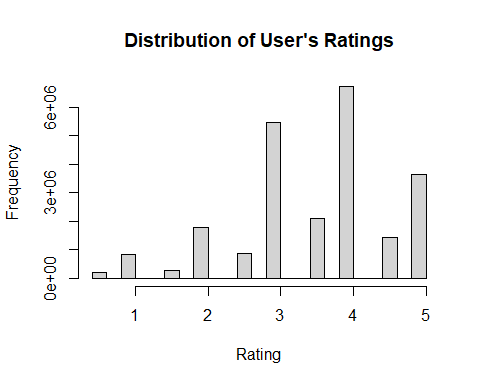
\includegraphics{MovieLens_Project_files/figure-latex/unnamed-chunk-16-1} \end{center}

\hypertarget{top-rated-movies}{%
\subsubsection{Top Rated Movies}\label{top-rated-movies}}

\begin{center}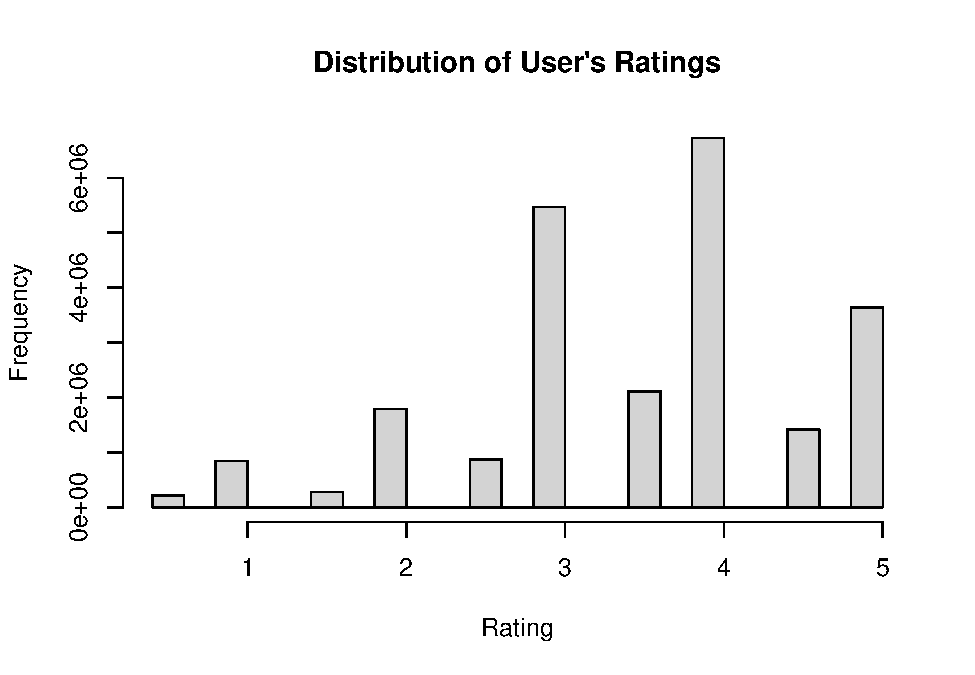
\includegraphics{MovieLens_Project_files/figure-latex/unnamed-chunk-17-1} \end{center}

\begin{table}[H]
\centering\begingroup\fontsize{10}{12}\selectfont

\begin{tabular}{l|r}
\hline
title & count\\
\hline
Forrest Gump & 124304\\
\hline
Toy Story & 119130\\
\hline
Jurassic Park & 117164\\
\hline
True Lies & 113930\\
\hline
Aladdin & 106070\\
\hline
Batman & 98656\\
\hline
Lion King, The & 94435\\
\hline
Pulp Fiction & 94008\\
\hline
Independence Day (a.k.a. ID4) & 93440\\
\hline
Silence of the Lambs, The & 90840\\
\hline
Beauty and the Beast & 89315\\
\hline
Fargo & 85480\\
\hline
Seven (a.k.a. Se7en) & 81084\\
\hline
Braveheart & 78774\\
\hline
Shrek & 78564\\
\hline
Star Wars: Episode IV - A New Hope (a.k.a. Star Wars) & 77427\\
\hline
Ghost & 77335\\
\hline
Who Framed Roger Rabbit? & 76825\\
\hline
Mission: Impossible & 75876\\
\hline
Princess Bride, The & 74045\\
\hline
Dances with Wolves & 69936\\
\hline
Blade Runner & 69615\\
\hline
Batman Forever & 69432\\
\hline
Mask, The & 68200\\
\hline
Babe & 68140\\
\hline
\end{tabular}
\endgroup{}
\end{table}

\hypertarget{mean-distribution-per-title}{%
\subsubsection{Mean Distribution per
Title}\label{mean-distribution-per-title}}

\begin{verbatim}
## # A tibble: 25 x 2
##    title                                                               mean
##    <chr>                                                              <dbl>
##  1 Blue Light, The (Das Blaue Licht)                                   5   
##  2 Constantine's Sword                                                 5   
##  3 Fighting Elegy (Kenka erejii)                                       5   
##  4 Hellhounds on My Trail                                              5   
##  5 Satan's Tango (Sátántangó)                                       5   
##  6 Shadows of Forgotten Ancestors                                      5   
##  7 Sun Alley (Sonnenallee)                                             5   
##  8 Human Condition II, The (Ningen no joken II)                        4.83
##  9 Human Condition III, The (Ningen no joken III)                      4.75
## 10 Who's Singin' Over There? (a.k.a. Who Sings Over There) (Ko to ta~  4.75
## # ... with 15 more rows
\end{verbatim}

\begin{center}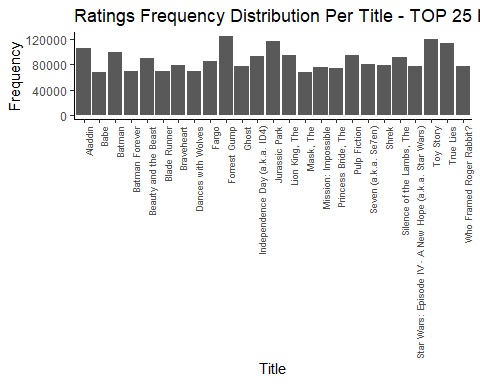
\includegraphics{MovieLens_Project_files/figure-latex/unnamed-chunk-19-1} \end{center}

\begin{table}[H]
\centering\begingroup\fontsize{10}{12}\selectfont

\begin{tabular}{l|r}
\hline
title & mean\\
\hline
Blue Light, The (Das Blaue Licht) & 5.000000\\
\hline
Constantine's Sword & 5.000000\\
\hline
Fighting Elegy (Kenka erejii) & 5.000000\\
\hline
Hellhounds on My Trail & 5.000000\\
\hline
Satan's Tango (Sátántangó) & 5.000000\\
\hline
Shadows of Forgotten Ancestors & 5.000000\\
\hline
Sun Alley (Sonnenallee) & 5.000000\\
\hline
Human Condition II, The (Ningen no joken II) & 4.833333\\
\hline
Human Condition III, The (Ningen no joken III) & 4.750000\\
\hline
Who's Singin' Over There? (a.k.a. Who Sings Over There) (Ko to tamo peva) & 4.750000\\
\hline
Class, The (Entre les Murs) & 4.666667\\
\hline
I'm Starting From Three (Ricomincio da Tre) & 4.666667\\
\hline
Man Who Planted Trees, The (Homme qui plantait des arbres, L') & 4.571429\\
\hline
Bad Blood (Mauvais sang) & 4.500000\\
\hline
Caótica Ana & 4.500000\\
\hline
Demon Lover Diary & 4.500000\\
\hline
End of Summer, The (Kohayagawa-ke no aki) & 4.500000\\
\hline
Fires on the Plain (Nobi) & 4.500000\\
\hline
Ladrones & 4.500000\\
\hline
Life of Oharu, The (Saikaku ichidai onna) & 4.500000\\
\hline
Man Named Pearl, A & 4.500000\\
\hline
Mickey & 4.500000\\
\hline
Please Vote for Me & 4.500000\\
\hline
Power of Nightmares: The Rise of the Politics of Fear, The & 4.500000\\
\hline
Testament of Orpheus, The (Testament d'Orphée) & 4.500000\\
\hline
\end{tabular}
\endgroup{}
\end{table}

\hypertarget{median-distribution-per-title}{%
\subsubsection{Median Distribution per
Title}\label{median-distribution-per-title}}

\begin{verbatim}
## # A tibble: 25 x 2
##    title                                                median
##    <chr>                                                 <dbl>
##  1 'burbs, The                                             3  
##  2 'night Mother                                           3.5
##  3 'Round Midnight                                         4  
##  4 'Til There Was You                                      3  
##  5 "\"Great Performances\" Cats"                           4  
##  6 *batteries not included                                 3  
##  7 ...All the Marbles (a.k.a. The California Dolls)        2  
##  8 ...And God Created Woman (Et Dieu... créa la femme)    3  
##  9 ...And God Spoke                                        3.5
## 10 ...And Justice for All                                  4  
## # ... with 15 more rows
\end{verbatim}

\begin{center}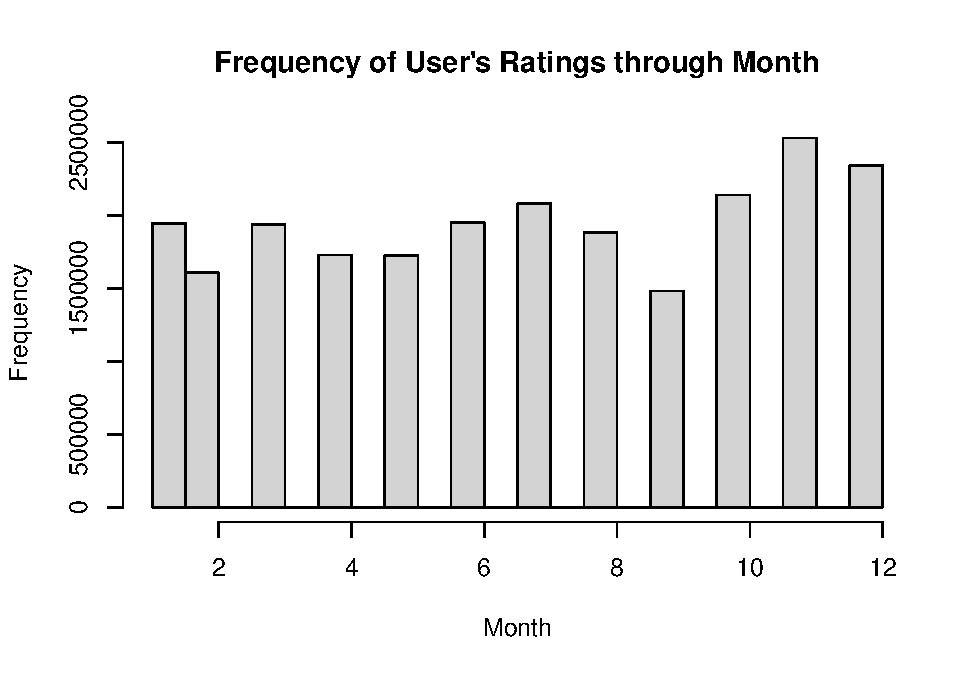
\includegraphics{MovieLens_Project_files/figure-latex/unnamed-chunk-21-1} \end{center}

\begin{table}[H]
\centering\begingroup\fontsize{10}{12}\selectfont

\begin{tabular}{l|r}
\hline
genre & median\\
\hline
Animation & 4.0\\
\hline
Crime & 4.0\\
\hline
Documentary & 4.0\\
\hline
Drama & 4.0\\
\hline
Film-Noir & 4.0\\
\hline
IMAX & 4.0\\
\hline
Musical & 4.0\\
\hline
Mystery & 4.0\\
\hline
Romance & 4.0\\
\hline
War & 4.0\\
\hline
Western & 4.0\\
\hline
(no genres listed) & 3.5\\
\hline
Action & 3.5\\
\hline
Adventure & 3.5\\
\hline
Children & 3.5\\
\hline
Comedy & 3.5\\
\hline
Fantasy & 3.5\\
\hline
Horror & 3.5\\
\hline
Sci-Fi & 3.5\\
\hline
Thriller & 3.5\\
\hline
\end{tabular}
\endgroup{}
\end{table}

\hypertarget{genre-analysis}{%
\subsection{Genre Analysis}\label{genre-analysis}}

\hypertarget{rating-distribution-per-genre}{%
\subsubsection{Rating Distribution per
Genre}\label{rating-distribution-per-genre}}

\textbf{Overview of Rating distribution over Genre}

\begin{center}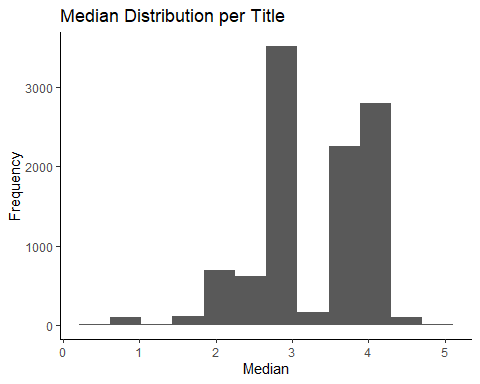
\includegraphics{MovieLens_Project_files/figure-latex/unnamed-chunk-23-1} \end{center}

\begin{Shaded}
\begin{Highlighting}[]
\NormalTok{edx }\OperatorTok
\StringTok{   }\KeywordTok{group_by}\NormalTok{(genre) }\OperatorTok
\StringTok{   }\KeywordTok{summarise}\NormalTok{(}\DataTypeTok{count =} \KeywordTok{n}\NormalTok{()) }\OperatorTok
\StringTok{   }\KeywordTok{arrange}\NormalTok{(}\KeywordTok{desc}\NormalTok{(count)) }\OperatorTok
\StringTok{   }\KeywordTok{kable}\NormalTok{() }\OperatorTok
\StringTok{   }\KeywordTok{kable_styling}\NormalTok{(}\DataTypeTok{bootstrap_options =} \KeywordTok{c}\NormalTok{(}\StringTok{"striped"}\NormalTok{, }\StringTok{"hover"}\NormalTok{, }\StringTok{"condensed"}\NormalTok{, }\StringTok{"responsive"}\NormalTok{),}
                 \DataTypeTok{position =} \StringTok{"center"}\NormalTok{,}
                 \DataTypeTok{font_size =} \DecValTok{10}\NormalTok{,}
                 \DataTypeTok{full_width =} \OtherTok{FALSE}\NormalTok{)}
\end{Highlighting}
\end{Shaded}

\begin{table}[H]
\centering\begingroup\fontsize{10}{12}\selectfont

\begin{tabular}{l|r}
\hline
genre & count\\
\hline
Drama & 3909401\\
\hline
Comedy & 3541284\\
\hline
Action & 2560649\\
\hline
Thriller & 2325349\\
\hline
Adventure & 1908692\\
\hline
Romance & 1712232\\
\hline
Sci-Fi & 1341750\\
\hline
Crime & 1326917\\
\hline
Fantasy & 925624\\
\hline
Children & 737851\\
\hline
Horror & 691407\\
\hline
Mystery & 567865\\
\hline
War & 511330\\
\hline
Animation & 467220\\
\hline
Musical & 432960\\
\hline
Western & 189234\\
\hline
Film-Noir & 118394\\
\hline
Documentary & 93252\\
\hline
IMAX & 8190\\
\hline
(no genres listed) & 6\\
\hline
\end{tabular}
\endgroup{}
\end{table}

\hypertarget{mean-distribution-per-genre}{%
\subsubsection{Mean Distribution per
Genre}\label{mean-distribution-per-genre}}

\begin{center}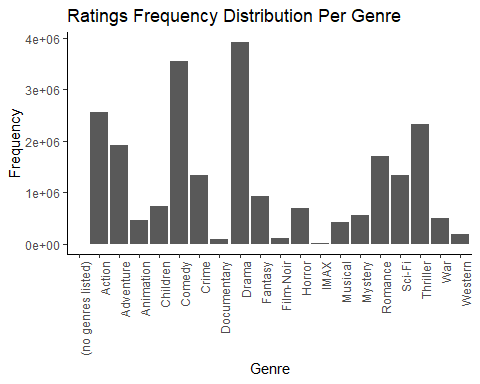
\includegraphics{MovieLens_Project_files/figure-latex/unnamed-chunk-25-1} \end{center}

\begin{table}[H]
\centering\begingroup\fontsize{10}{12}\selectfont

\begin{tabular}{l|r}
\hline
genre & mean\\
\hline
Film-Noir & 4.011732\\
\hline
Documentary & 3.784385\\
\hline
War & 3.779457\\
\hline
IMAX & 3.761844\\
\hline
Mystery & 3.677412\\
\hline
Drama & 3.673047\\
\hline
Crime & 3.666151\\
\hline
Animation & 3.599588\\
\hline
Musical & 3.562761\\
\hline
Western & 3.555122\\
\hline
Romance & 3.553594\\
\hline
Thriller & 3.506879\\
\hline
Fantasy & 3.502419\\
\hline
(no genres listed) & 3.500000\\
\hline
Adventure & 3.494076\\
\hline
Comedy & 3.437040\\
\hline
Action & 3.421589\\
\hline
Children & 3.418673\\
\hline
Sci-Fi & 3.396756\\
\hline
Horror & 3.269523\\
\hline
\end{tabular}
\endgroup{}
\end{table}

\hypertarget{median-distribution-per-genre}{%
\subsubsection{Median Distribution per
Genre}\label{median-distribution-per-genre}}

\begin{center}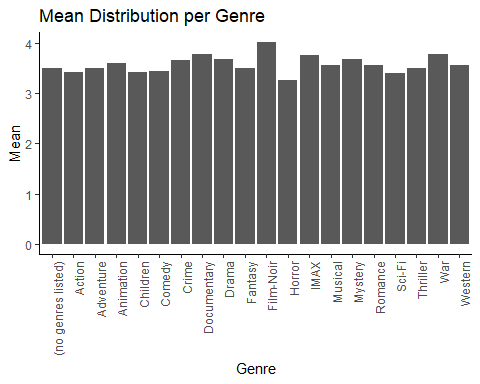
\includegraphics{MovieLens_Project_files/figure-latex/unnamed-chunk-27-1} \end{center}

\begin{table}[H]
\centering\begingroup\fontsize{10}{12}\selectfont

\begin{tabular}{l|r}
\hline
genre & median\\
\hline
Animation & 4.0\\
\hline
Crime & 4.0\\
\hline
Documentary & 4.0\\
\hline
Drama & 4.0\\
\hline
Film-Noir & 4.0\\
\hline
IMAX & 4.0\\
\hline
Musical & 4.0\\
\hline
Mystery & 4.0\\
\hline
Romance & 4.0\\
\hline
War & 4.0\\
\hline
Western & 4.0\\
\hline
(no genres listed) & 3.5\\
\hline
Action & 3.5\\
\hline
Adventure & 3.5\\
\hline
Children & 3.5\\
\hline
Comedy & 3.5\\
\hline
Fantasy & 3.5\\
\hline
Horror & 3.5\\
\hline
Sci-Fi & 3.5\\
\hline
Thriller & 3.5\\
\hline
\end{tabular}
\endgroup{}
\end{table}

\hypertarget{analysis---model-building-and-evaluation}{%
\section{Analysis - Model Building and
Evaluation}\label{analysis---model-building-and-evaluation}}

\hypertarget{naive-baseline-model}{%
\subsection{Naive Baseline Model}\label{naive-baseline-model}}

The simplest model that someone can build, is a Naive Model that predict
ALWAYS the mean or the median. In this case, the mean is approximately
3.5 and the median is 4.

\begin{Shaded}
\begin{Highlighting}[]
\KeywordTok{paste}\NormalTok{(}\StringTok{"The mean is:"}\NormalTok{, }\KeywordTok{as.character}\NormalTok{(}\KeywordTok{mean}\NormalTok{(edx}\OperatorTok{$}\NormalTok{rating)))}
\end{Highlighting}
\end{Shaded}

\begin{verbatim}
## [1] "The mean is: 3.52700364195256"
\end{verbatim}

\begin{Shaded}
\begin{Highlighting}[]
\KeywordTok{paste}\NormalTok{(}\StringTok{"The median is:"}\NormalTok{, }\KeywordTok{as.character}\NormalTok{(}\KeywordTok{median}\NormalTok{(edx}\OperatorTok{$}\NormalTok{rating)))}
\end{Highlighting}
\end{Shaded}

\begin{verbatim}
## [1] "The median is: 4"
\end{verbatim}

\[Y_{u,i} = \tilde{\chi} + \varepsilon_{u,i}\]

With \(\tilde{\chi}\) is the median and \(\varepsilon_{i,u}\)
independent errors sampled from the same distribution.

\hypertarget{naive-mean-baseline-model}{%
\subsubsection{Naive Mean-Baseline
Model}\label{naive-mean-baseline-model}}

The formula used is:

\[Y_{u,i} = \mu + \varepsilon_{u,i}\]

With \(\mu\) is the mean and \(\varepsilon_{i,u}\) independent errors
sampled from the same distribution.

\hypertarget{naive-median-baseline-model}{%
\subsubsection{Naive Median-Baseline
Model}\label{naive-median-baseline-model}}

The formula used is:

\[Y_{u,i} = \tilde{\chi} + \varepsilon_{u,i}\]

With \(\tilde{\chi}\) is the median and \(\varepsilon_{i,u}\)
independent errors sampled from the same distribution centered at 0.

\hypertarget{movie-based-model-a-content-based-approach}{%
\subsection{Movie-Based Model, a Content-based
Approach}\label{movie-based-model-a-content-based-approach}}

\hypertarget{movie-user-model-a-user-based-approach}{%
\subsection{Movie + User Model, a User-based
approach}\label{movie-user-model-a-user-based-approach}}

\hypertarget{regularization}{%
\subsection{Regularization}\label{regularization}}

\hypertarget{regularized-movie-based-model}{%
\subsubsection{Regularized Movie-Based
Model}\label{regularized-movie-based-model}}

\hypertarget{regularized-user-based-model}{%
\subsubsection{Regularized User-Based
Model}\label{regularized-user-based-model}}

\hypertarget{results-and-conclusion}{%
\section{Results and Conclusion}\label{results-and-conclusion}}

\hypertarget{appendix}{%
\section{Appendix}\label{appendix}}

\hypertarget{a---initial-code-privided-by-edx}{%
\subsection{1a - Initial Code privided by
edX}\label{a---initial-code-privided-by-edx}}

\begin{verbatim}
#############################################################
# Create edx set, validation set, and submission file
#############################################################

# Note: this process could take a couple of minutes

if(!require(tidyverse)) install.packages("tidyverse", repos = "http://cran.us.r-project.org")
if(!require(caret)) install.packages("caret", repos = "http://cran.us.r-project.org")

# MovieLens 10M dataset:
# https://grouplens.org/datasets/movielens/10m/
# http://files.grouplens.org/datasets/movielens/ml-10m.zip

dl <- tempfile()
download.file("http://files.grouplens.org/datasets/movielens/ml-10m.zip", dl)

ratings <- read.table(text = gsub("::", "\t", readLines(unzip(dl, "ml-10M100K/ratings.dat"))),
                      col.names = c("userId", "movieId", "rating", "timestamp"))

movies <- str_split_fixed(readLines(unzip(dl, "ml-10M100K/movies.dat")), "\\::", 3)
colnames(movies) <- c("movieId", "title", "genres")
movies <- as.data.frame(movies) %>% mutate(movieId = as.numeric(levels(movieId))[movieId],
                                           title = as.character(title),
                                           genres = as.character(genres))

movielens <- left_join(ratings, movies, by = "movieId")

# Validation set will be 10% of MovieLens data

set.seed(1)
test_index <- createDataPartition(y = movielens$rating, times = 1, p = 0.1, list = FALSE)
edx <- movielens[-test_index,]
temp <- movielens[test_index,]

# Make sure userId and movieId in validation set are also in edx set

validation <- temp %>% 
  semi_join(edx, by = "movieId") %>%
  semi_join(edx, by = "userId")

# Add rows removed from validation set back into edx set

removed <- anti_join(temp, validation)
edx <- rbind(edx, removed)

rm(dl, ratings, movies, test_index, temp, movielens, removed)
write.csv(edx, "edx.csv")
\end{verbatim}

\hypertarget{b---code-used-in-this-report}{%
\subsection{1b - Code used in this
report}\label{b---code-used-in-this-report}}

\hypertarget{c---enviroment}{%
\subsection{1c - Enviroment}\label{c---enviroment}}

\begin{Shaded}
\begin{Highlighting}[]
\KeywordTok{print}\NormalTok{(}\StringTok{"Operating System:"}\NormalTok{)}
\end{Highlighting}
\end{Shaded}

\begin{verbatim}
## [1] "Operating System:"
\end{verbatim}

\begin{Shaded}
\begin{Highlighting}[]
\NormalTok{version}
\end{Highlighting}
\end{Shaded}

\begin{verbatim}
##                _                           
## platform       x86_64-w64-mingw32          
## arch           x86_64                      
## os             mingw32                     
## system         x86_64, mingw32             
## status                                     
## major          3                           
## minor          6.0                         
## year           2019                        
## month          04                          
## day            26                          
## svn rev        76424                       
## language       R                           
## version.string R version 3.6.0 (2019-04-26)
## nickname       Planting of a Tree
\end{verbatim}

\begin{Shaded}
\begin{Highlighting}[]
\KeywordTok{print}\NormalTok{(}\StringTok{"All installed packages"}\NormalTok{)}
\end{Highlighting}
\end{Shaded}

\begin{verbatim}
## [1] "All installed packages"
\end{verbatim}

\begin{Shaded}
\begin{Highlighting}[]
\KeywordTok{installed.packages}\NormalTok{()}
\end{Highlighting}
\end{Shaded}

\begin{verbatim}
##              Package       
## askpass      "askpass"     
## assertthat   "assertthat"  
## backports    "backports"   
## base64enc    "base64enc"   
## BH           "BH"          
## bitops       "bitops"      
## broom        "broom"       
## callr        "callr"       
## caret        "caret"       
## caTools      "caTools"     
## cellranger   "cellranger"  
## cli          "cli"         
## clipr        "clipr"       
## colorspace   "colorspace"  
## crayon       "crayon"      
## curl         "curl"        
## data.table   "data.table"  
## DBI          "DBI"         
## dbplyr       "dbplyr"      
## digest       "digest"      
## dplyr        "dplyr"       
## dslabs       "dslabs"      
## ellipsis     "ellipsis"    
## evaluate     "evaluate"    
## fansi        "fansi"       
## forcats      "forcats"     
## foreach      "foreach"     
## fs           "fs"          
## generics     "generics"    
## ggplot2      "ggplot2"     
## glue         "glue"        
## gower        "gower"       
## gtable       "gtable"      
## haven        "haven"       
## highr        "highr"       
## hms          "hms"         
## htmltools    "htmltools"   
## httr         "httr"        
## ipred        "ipred"       
## iterators    "iterators"   
## jsonlite     "jsonlite"    
## kableExtra   "kableExtra"  
## knitr        "knitr"       
## labeling     "labeling"    
## lava         "lava"        
## lazyeval     "lazyeval"    
## lubridate    "lubridate"   
## magrittr     "magrittr"    
## markdown     "markdown"    
## mime         "mime"        
## ModelMetrics "ModelMetrics"
## modelr       "modelr"      
## munsell      "munsell"     
## numDeriv     "numDeriv"    
## openssl      "openssl"     
## pillar       "pillar"      
## pkgconfig    "pkgconfig"   
## plogr        "plogr"       
## plyr         "plyr"        
## prettyunits  "prettyunits" 
## processx     "processx"    
## prodlim      "prodlim"     
## progress     "progress"    
## ps           "ps"          
## purrr        "purrr"       
## R6           "R6"          
## RColorBrewer "RColorBrewer"
## Rcpp         "Rcpp"        
## RcppRoll     "RcppRoll"    
## readr        "readr"       
## readxl       "readxl"      
## recipes      "recipes"     
## rematch      "rematch"     
## reprex       "reprex"      
## reshape2     "reshape2"    
## rlang        "rlang"       
## rmarkdown    "rmarkdown"   
## rprojroot    "rprojroot"   
## rstudioapi   "rstudioapi"  
## rvest        "rvest"       
## scales       "scales"      
## selectr      "selectr"     
## SQUAREM      "SQUAREM"     
## stringi      "stringi"     
## stringr      "stringr"     
## sys          "sys"         
## tibble       "tibble"      
## tidyr        "tidyr"       
## tidyselect   "tidyselect"  
## tidyverse    "tidyverse"   
## timeDate     "timeDate"    
## tinytex      "tinytex"     
## utf8         "utf8"        
## viridisLite  "viridisLite" 
## webshot      "webshot"     
## whisker      "whisker"     
## withr        "withr"       
## xfun         "xfun"        
## xml2         "xml2"        
## yaml         "yaml"        
## base         "base"        
## boot         "boot"        
## class        "class"       
## cluster      "cluster"     
## codetools    "codetools"   
## compiler     "compiler"    
## datasets     "datasets"    
## foreign      "foreign"     
## graphics     "graphics"    
## grDevices    "grDevices"   
## grid         "grid"        
## KernSmooth   "KernSmooth"  
## lattice      "lattice"     
## MASS         "MASS"        
## Matrix       "Matrix"      
## methods      "methods"     
## mgcv         "mgcv"        
## nlme         "nlme"        
## nnet         "nnet"        
## parallel     "parallel"    
## rpart        "rpart"       
## spatial      "spatial"     
## splines      "splines"     
## stats        "stats"       
## stats4       "stats4"      
## survival     "survival"    
## tcltk        "tcltk"       
## tools        "tools"       
## translations "translations"
## utils        "utils"       
##              LibPath                                              
## askpass      "C:/Users/aless/OneDrive/Documenti/R/win-library/3.6"
## assertthat   "C:/Users/aless/OneDrive/Documenti/R/win-library/3.6"
## backports    "C:/Users/aless/OneDrive/Documenti/R/win-library/3.6"
## base64enc    "C:/Users/aless/OneDrive/Documenti/R/win-library/3.6"
## BH           "C:/Users/aless/OneDrive/Documenti/R/win-library/3.6"
## bitops       "C:/Users/aless/OneDrive/Documenti/R/win-library/3.6"
## broom        "C:/Users/aless/OneDrive/Documenti/R/win-library/3.6"
## callr        "C:/Users/aless/OneDrive/Documenti/R/win-library/3.6"
## caret        "C:/Users/aless/OneDrive/Documenti/R/win-library/3.6"
## caTools      "C:/Users/aless/OneDrive/Documenti/R/win-library/3.6"
## cellranger   "C:/Users/aless/OneDrive/Documenti/R/win-library/3.6"
## cli          "C:/Users/aless/OneDrive/Documenti/R/win-library/3.6"
## clipr        "C:/Users/aless/OneDrive/Documenti/R/win-library/3.6"
## colorspace   "C:/Users/aless/OneDrive/Documenti/R/win-library/3.6"
## crayon       "C:/Users/aless/OneDrive/Documenti/R/win-library/3.6"
## curl         "C:/Users/aless/OneDrive/Documenti/R/win-library/3.6"
## data.table   "C:/Users/aless/OneDrive/Documenti/R/win-library/3.6"
## DBI          "C:/Users/aless/OneDrive/Documenti/R/win-library/3.6"
## dbplyr       "C:/Users/aless/OneDrive/Documenti/R/win-library/3.6"
## digest       "C:/Users/aless/OneDrive/Documenti/R/win-library/3.6"
## dplyr        "C:/Users/aless/OneDrive/Documenti/R/win-library/3.6"
## dslabs       "C:/Users/aless/OneDrive/Documenti/R/win-library/3.6"
## ellipsis     "C:/Users/aless/OneDrive/Documenti/R/win-library/3.6"
## evaluate     "C:/Users/aless/OneDrive/Documenti/R/win-library/3.6"
## fansi        "C:/Users/aless/OneDrive/Documenti/R/win-library/3.6"
## forcats      "C:/Users/aless/OneDrive/Documenti/R/win-library/3.6"
## foreach      "C:/Users/aless/OneDrive/Documenti/R/win-library/3.6"
## fs           "C:/Users/aless/OneDrive/Documenti/R/win-library/3.6"
## generics     "C:/Users/aless/OneDrive/Documenti/R/win-library/3.6"
## ggplot2      "C:/Users/aless/OneDrive/Documenti/R/win-library/3.6"
## glue         "C:/Users/aless/OneDrive/Documenti/R/win-library/3.6"
## gower        "C:/Users/aless/OneDrive/Documenti/R/win-library/3.6"
## gtable       "C:/Users/aless/OneDrive/Documenti/R/win-library/3.6"
## haven        "C:/Users/aless/OneDrive/Documenti/R/win-library/3.6"
## highr        "C:/Users/aless/OneDrive/Documenti/R/win-library/3.6"
## hms          "C:/Users/aless/OneDrive/Documenti/R/win-library/3.6"
## htmltools    "C:/Users/aless/OneDrive/Documenti/R/win-library/3.6"
## httr         "C:/Users/aless/OneDrive/Documenti/R/win-library/3.6"
## ipred        "C:/Users/aless/OneDrive/Documenti/R/win-library/3.6"
## iterators    "C:/Users/aless/OneDrive/Documenti/R/win-library/3.6"
## jsonlite     "C:/Users/aless/OneDrive/Documenti/R/win-library/3.6"
## kableExtra   "C:/Users/aless/OneDrive/Documenti/R/win-library/3.6"
## knitr        "C:/Users/aless/OneDrive/Documenti/R/win-library/3.6"
## labeling     "C:/Users/aless/OneDrive/Documenti/R/win-library/3.6"
## lava         "C:/Users/aless/OneDrive/Documenti/R/win-library/3.6"
## lazyeval     "C:/Users/aless/OneDrive/Documenti/R/win-library/3.6"
## lubridate    "C:/Users/aless/OneDrive/Documenti/R/win-library/3.6"
## magrittr     "C:/Users/aless/OneDrive/Documenti/R/win-library/3.6"
## markdown     "C:/Users/aless/OneDrive/Documenti/R/win-library/3.6"
## mime         "C:/Users/aless/OneDrive/Documenti/R/win-library/3.6"
## ModelMetrics "C:/Users/aless/OneDrive/Documenti/R/win-library/3.6"
## modelr       "C:/Users/aless/OneDrive/Documenti/R/win-library/3.6"
## munsell      "C:/Users/aless/OneDrive/Documenti/R/win-library/3.6"
## numDeriv     "C:/Users/aless/OneDrive/Documenti/R/win-library/3.6"
## openssl      "C:/Users/aless/OneDrive/Documenti/R/win-library/3.6"
## pillar       "C:/Users/aless/OneDrive/Documenti/R/win-library/3.6"
## pkgconfig    "C:/Users/aless/OneDrive/Documenti/R/win-library/3.6"
## plogr        "C:/Users/aless/OneDrive/Documenti/R/win-library/3.6"
## plyr         "C:/Users/aless/OneDrive/Documenti/R/win-library/3.6"
## prettyunits  "C:/Users/aless/OneDrive/Documenti/R/win-library/3.6"
## processx     "C:/Users/aless/OneDrive/Documenti/R/win-library/3.6"
## prodlim      "C:/Users/aless/OneDrive/Documenti/R/win-library/3.6"
## progress     "C:/Users/aless/OneDrive/Documenti/R/win-library/3.6"
## ps           "C:/Users/aless/OneDrive/Documenti/R/win-library/3.6"
## purrr        "C:/Users/aless/OneDrive/Documenti/R/win-library/3.6"
## R6           "C:/Users/aless/OneDrive/Documenti/R/win-library/3.6"
## RColorBrewer "C:/Users/aless/OneDrive/Documenti/R/win-library/3.6"
## Rcpp         "C:/Users/aless/OneDrive/Documenti/R/win-library/3.6"
## RcppRoll     "C:/Users/aless/OneDrive/Documenti/R/win-library/3.6"
## readr        "C:/Users/aless/OneDrive/Documenti/R/win-library/3.6"
## readxl       "C:/Users/aless/OneDrive/Documenti/R/win-library/3.6"
## recipes      "C:/Users/aless/OneDrive/Documenti/R/win-library/3.6"
## rematch      "C:/Users/aless/OneDrive/Documenti/R/win-library/3.6"
## reprex       "C:/Users/aless/OneDrive/Documenti/R/win-library/3.6"
## reshape2     "C:/Users/aless/OneDrive/Documenti/R/win-library/3.6"
## rlang        "C:/Users/aless/OneDrive/Documenti/R/win-library/3.6"
## rmarkdown    "C:/Users/aless/OneDrive/Documenti/R/win-library/3.6"
## rprojroot    "C:/Users/aless/OneDrive/Documenti/R/win-library/3.6"
## rstudioapi   "C:/Users/aless/OneDrive/Documenti/R/win-library/3.6"
## rvest        "C:/Users/aless/OneDrive/Documenti/R/win-library/3.6"
## scales       "C:/Users/aless/OneDrive/Documenti/R/win-library/3.6"
## selectr      "C:/Users/aless/OneDrive/Documenti/R/win-library/3.6"
## SQUAREM      "C:/Users/aless/OneDrive/Documenti/R/win-library/3.6"
## stringi      "C:/Users/aless/OneDrive/Documenti/R/win-library/3.6"
## stringr      "C:/Users/aless/OneDrive/Documenti/R/win-library/3.6"
## sys          "C:/Users/aless/OneDrive/Documenti/R/win-library/3.6"
## tibble       "C:/Users/aless/OneDrive/Documenti/R/win-library/3.6"
## tidyr        "C:/Users/aless/OneDrive/Documenti/R/win-library/3.6"
## tidyselect   "C:/Users/aless/OneDrive/Documenti/R/win-library/3.6"
## tidyverse    "C:/Users/aless/OneDrive/Documenti/R/win-library/3.6"
## timeDate     "C:/Users/aless/OneDrive/Documenti/R/win-library/3.6"
## tinytex      "C:/Users/aless/OneDrive/Documenti/R/win-library/3.6"
## utf8         "C:/Users/aless/OneDrive/Documenti/R/win-library/3.6"
## viridisLite  "C:/Users/aless/OneDrive/Documenti/R/win-library/3.6"
## webshot      "C:/Users/aless/OneDrive/Documenti/R/win-library/3.6"
## whisker      "C:/Users/aless/OneDrive/Documenti/R/win-library/3.6"
## withr        "C:/Users/aless/OneDrive/Documenti/R/win-library/3.6"
## xfun         "C:/Users/aless/OneDrive/Documenti/R/win-library/3.6"
## xml2         "C:/Users/aless/OneDrive/Documenti/R/win-library/3.6"
## yaml         "C:/Users/aless/OneDrive/Documenti/R/win-library/3.6"
## base         "C:/Program Files/R/R-3.6.0/library"                 
## boot         "C:/Program Files/R/R-3.6.0/library"                 
## class        "C:/Program Files/R/R-3.6.0/library"                 
## cluster      "C:/Program Files/R/R-3.6.0/library"                 
## codetools    "C:/Program Files/R/R-3.6.0/library"                 
## compiler     "C:/Program Files/R/R-3.6.0/library"                 
## datasets     "C:/Program Files/R/R-3.6.0/library"                 
## foreign      "C:/Program Files/R/R-3.6.0/library"                 
## graphics     "C:/Program Files/R/R-3.6.0/library"                 
## grDevices    "C:/Program Files/R/R-3.6.0/library"                 
## grid         "C:/Program Files/R/R-3.6.0/library"                 
## KernSmooth   "C:/Program Files/R/R-3.6.0/library"                 
## lattice      "C:/Program Files/R/R-3.6.0/library"                 
## MASS         "C:/Program Files/R/R-3.6.0/library"                 
## Matrix       "C:/Program Files/R/R-3.6.0/library"                 
## methods      "C:/Program Files/R/R-3.6.0/library"                 
## mgcv         "C:/Program Files/R/R-3.6.0/library"                 
## nlme         "C:/Program Files/R/R-3.6.0/library"                 
## nnet         "C:/Program Files/R/R-3.6.0/library"                 
## parallel     "C:/Program Files/R/R-3.6.0/library"                 
## rpart        "C:/Program Files/R/R-3.6.0/library"                 
## spatial      "C:/Program Files/R/R-3.6.0/library"                 
## splines      "C:/Program Files/R/R-3.6.0/library"                 
## stats        "C:/Program Files/R/R-3.6.0/library"                 
## stats4       "C:/Program Files/R/R-3.6.0/library"                 
## survival     "C:/Program Files/R/R-3.6.0/library"                 
## tcltk        "C:/Program Files/R/R-3.6.0/library"                 
## tools        "C:/Program Files/R/R-3.6.0/library"                 
## translations "C:/Program Files/R/R-3.6.0/library"                 
## utils        "C:/Program Files/R/R-3.6.0/library"                 
##              Version      Priority     
## askpass      "1.1"        NA           
## assertthat   "0.2.1"      NA           
## backports    "1.1.4"      NA           
## base64enc    "0.1-3"      NA           
## BH           "1.69.0-1"   NA           
## bitops       "1.0-6"      NA           
## broom        "0.5.2"      NA           
## callr        "3.2.0"      NA           
## caret        "6.0-84"     NA           
## caTools      "1.17.1.2"   NA           
## cellranger   "1.1.0"      NA           
## cli          "1.1.0"      NA           
## clipr        "0.6.0"      NA           
## colorspace   "1.4-1"      NA           
## crayon       "1.3.4"      NA           
## curl         "3.3"        NA           
## data.table   "1.12.2"     NA           
## DBI          "1.0.0"      NA           
## dbplyr       "1.4.0"      NA           
## digest       "0.6.18"     NA           
## dplyr        "0.8.0.1"    NA           
## dslabs       "0.5.2"      NA           
## ellipsis     "0.1.0"      NA           
## evaluate     "0.13"       NA           
## fansi        "0.4.0"      NA           
## forcats      "0.4.0"      NA           
## foreach      "1.4.4"      NA           
## fs           "1.3.0"      NA           
## generics     "0.0.2"      NA           
## ggplot2      "3.1.1"      NA           
## glue         "1.3.1"      NA           
## gower        "0.2.0"      NA           
## gtable       "0.3.0"      NA           
## haven        "2.1.0"      NA           
## highr        "0.8"        NA           
## hms          "0.4.2"      NA           
## htmltools    "0.3.6"      NA           
## httr         "1.4.0"      NA           
## ipred        "0.9-9"      NA           
## iterators    "1.0.10"     NA           
## jsonlite     "1.6"        NA           
## kableExtra   "1.1.0"      NA           
## knitr        "1.22"       NA           
## labeling     "0.3"        NA           
## lava         "1.6.5"      NA           
## lazyeval     "0.2.2"      NA           
## lubridate    "1.7.4"      NA           
## magrittr     "1.5"        NA           
## markdown     "0.9"        NA           
## mime         "0.6"        NA           
## ModelMetrics "1.2.2"      NA           
## modelr       "0.1.4"      NA           
## munsell      "0.5.0"      NA           
## numDeriv     "2016.8-1"   NA           
## openssl      "1.3"        NA           
## pillar       "1.3.1"      NA           
## pkgconfig    "2.0.2"      NA           
## plogr        "0.2.0"      NA           
## plyr         "1.8.4"      NA           
## prettyunits  "1.0.2"      NA           
## processx     "3.3.0"      NA           
## prodlim      "2018.04.18" NA           
## progress     "1.2.0"      NA           
## ps           "1.3.0"      NA           
## purrr        "0.3.2"      NA           
## R6           "2.4.0"      NA           
## RColorBrewer "1.1-2"      NA           
## Rcpp         "1.0.1"      NA           
## RcppRoll     "0.3.0"      NA           
## readr        "1.3.1"      NA           
## readxl       "1.3.1"      NA           
## recipes      "0.1.5"      NA           
## rematch      "1.0.1"      NA           
## reprex       "0.2.1"      NA           
## reshape2     "1.4.3"      NA           
## rlang        "0.3.4"      NA           
## rmarkdown    "1.12"       NA           
## rprojroot    "1.3-2"      NA           
## rstudioapi   "0.10"       NA           
## rvest        "0.3.3"      NA           
## scales       "1.0.0"      NA           
## selectr      "0.4-1"      NA           
## SQUAREM      "2017.10-1"  NA           
## stringi      "1.4.3"      NA           
## stringr      "1.4.0"      NA           
## sys          "3.2"        NA           
## tibble       "2.1.1"      NA           
## tidyr        "0.8.3"      NA           
## tidyselect   "0.2.5"      NA           
## tidyverse    "1.2.1"      NA           
## timeDate     "3043.102"   NA           
## tinytex      "0.12"       NA           
## utf8         "1.1.4"      NA           
## viridisLite  "0.3.0"      NA           
## webshot      "0.5.1"      NA           
## whisker      "0.3-2"      NA           
## withr        "2.1.2"      NA           
## xfun         "0.6"        NA           
## xml2         "1.2.0"      NA           
## yaml         "2.2.0"      NA           
## base         "3.6.0"      "base"       
## boot         "1.3-22"     "recommended"
## class        "7.3-15"     "recommended"
## cluster      "2.0.8"      "recommended"
## codetools    "0.2-16"     "recommended"
## compiler     "3.6.0"      "base"       
## datasets     "3.6.0"      "base"       
## foreign      "0.8-71"     "recommended"
## graphics     "3.6.0"      "base"       
## grDevices    "3.6.0"      "base"       
## grid         "3.6.0"      "base"       
## KernSmooth   "2.23-15"    "recommended"
## lattice      "0.20-38"    "recommended"
## MASS         "7.3-51.4"   "recommended"
## Matrix       "1.2-17"     "recommended"
## methods      "3.6.0"      "base"       
## mgcv         "1.8-28"     "recommended"
## nlme         "3.1-139"    "recommended"
## nnet         "7.3-12"     "recommended"
## parallel     "3.6.0"      "base"       
## rpart        "4.1-15"     "recommended"
## spatial      "7.3-11"     "recommended"
## splines      "3.6.0"      "base"       
## stats        "3.6.0"      "base"       
## stats4       "3.6.0"      "base"       
## survival     "2.44-1.1"   "recommended"
## tcltk        "3.6.0"      "base"       
## tools        "3.6.0"      "base"       
## translations "3.6.0"      NA           
## utils        "3.6.0"      "base"       
##              Depends                                          
## askpass      NA                                               
## assertthat   NA                                               
## backports    "R (>= 3.0.0)"                                   
## base64enc    "R (>= 2.9.0)"                                   
## BH           NA                                               
## bitops       NA                                               
## broom        "R (>= 3.1)"                                     
## callr        NA                                               
## caret        "R (>= 3.2.0), lattice (>= 0.20), ggplot2"       
## caTools      "R (>= 2.2.0)"                                   
## cellranger   "R (>= 3.0.0)"                                   
## cli          "R (>= 2.10)"                                    
## clipr        NA                                               
## colorspace   "R (>= 3.0.0), methods"                          
## crayon       NA                                               
## curl         "R (>= 3.0.0)"                                   
## data.table   "R (>= 3.1.0)"                                   
## DBI          "R (>= 3.0.0), methods"                          
## dbplyr       "R (>= 3.1)"                                     
## digest       "R (>= 3.1.0)"                                   
## dplyr        "R (>= 3.1.2)"                                   
## dslabs       "R (>= 3.1.2)"                                   
## ellipsis     "R (>= 3.1)"                                     
## evaluate     "R (>= 3.0.2)"                                   
## fansi        "R (>= 3.1.0)"                                   
## forcats      "R (>= 3.1)"                                     
## foreach      "R (>= 2.5.0)"                                   
## fs           "R (>= 3.1)"                                     
## generics     "R (>= 3.1)"                                     
## ggplot2      "R (>= 3.1)"                                     
## glue         "R (>= 3.1)"                                     
## gower        NA                                               
## gtable       "R (>= 3.0)"                                     
## haven        "R (>= 3.1)"                                     
## highr        "R (>= 3.2.3)"                                   
## hms          NA                                               
## htmltools    "R (>= 2.14.1)"                                  
## httr         "R (>= 3.1)"                                     
## ipred        "R (>= 2.10)"                                    
## iterators    "R (>= 2.5.0), utils"                            
## jsonlite     "methods"                                        
## kableExtra   "R (>= 3.1.0)"                                   
## knitr        "R (>= 3.1.0)"                                   
## labeling     NA                                               
## lava         "R (>= 3.0)"                                     
## lazyeval     "R (>= 3.1.0)"                                   
## lubridate    "methods, R (>= 3.0.0)"                          
## magrittr     NA                                               
## markdown     "R (>= 2.11.1)"                                  
## mime         NA                                               
## ModelMetrics "R (>= 3.2.2)"                                   
## modelr       "R (>= 3.1)"                                     
## munsell      NA                                               
## numDeriv     "R (>= 2.11.1)"                                  
## openssl      NA                                               
## pillar       NA                                               
## pkgconfig    NA                                               
## plogr        NA                                               
## plyr         "R (>= 3.1.0)"                                   
## prettyunits  NA                                               
## processx     NA                                               
## prodlim      "R (>= 2.9.0)"                                   
## progress     NA                                               
## ps           "R (>= 3.1)"                                     
## purrr        "R (>= 3.1)"                                     
## R6           "R (>= 3.0)"                                     
## RColorBrewer "R (>= 2.0.0)"                                   
## Rcpp         "R (>= 3.0.0)"                                   
## RcppRoll     "R (>= 2.15.1)"                                  
## readr        "R (>= 3.1)"                                     
## readxl       NA                                               
## recipes      "R (>= 3.1), dplyr"                              
## rematch      NA                                               
## reprex       "R (>= 3.1)"                                     
## reshape2     "R (>= 3.1)"                                     
## rlang        "R (>= 3.1.0)"                                   
## rmarkdown    "R (>= 3.0)"                                     
## rprojroot    "R (>= 3.0.0)"                                   
## rstudioapi   NA                                               
## rvest        "R (>= 3.1), xml2"                               
## scales       "R (>= 3.1)"                                     
## selectr      "R (>= 3.0)"                                     
## SQUAREM      "R (>= 3.0)"                                     
## stringi      "R (>= 2.14)"                                    
## stringr      "R (>= 3.1)"                                     
## sys          NA                                               
## tibble       "R (>= 3.1.0)"                                   
## tidyr        "R (>= 3.1)"                                     
## tidyselect   "R (>= 3.1)"                                     
## tidyverse    NA                                               
## timeDate     "R (>= 2.15.1), graphics, utils, stats, methods" 
## tinytex      NA                                               
## utf8         "R (>= 2.10)"                                    
## viridisLite  "R (>= 2.10)"                                    
## webshot      "R (>= 3.0)"                                     
## whisker      NA                                               
## withr        "R (>= 3.0.2)"                                   
## xfun         NA                                               
## xml2         "R (>= 3.1.0)"                                   
## yaml         NA                                               
## base         NA                                               
## boot         "R (>= 3.0.0), graphics, stats"                  
## class        "R (>= 3.0.0), stats, utils"                     
## cluster      "R (>= 3.3.0)"                                   
## codetools    "R (>= 2.1)"                                     
## compiler     NA                                               
## datasets     NA                                               
## foreign      "R (>= 3.0.0)"                                   
## graphics     NA                                               
## grDevices    NA                                               
## grid         NA                                               
## KernSmooth   "R (>= 2.5.0), stats"                            
## lattice      "R (>= 3.0.0)"                                   
## MASS         "R (>= 3.1.0), grDevices, graphics, stats, utils"
## Matrix       "R (>= 3.2.0)"                                   
## methods      NA                                               
## mgcv         "R (>= 2.14.0), nlme (>= 3.1-64)"                
## nlme         "R (>= 3.4.0)"                                   
## nnet         "R (>= 2.14.0), stats, utils"                    
## parallel     NA                                               
## rpart        "R (>= 2.15.0), graphics, stats, grDevices"      
## spatial      "R (>= 3.0.0), graphics, stats, utils"           
## splines      NA                                               
## stats        NA                                               
## stats4       NA                                               
## survival     "R (>= 2.13.0)"                                  
## tcltk        NA                                               
## tools        NA                                               
## translations NA                                               
## utils        NA                                               
##              Imports                                                                                                                                                                                                                                                                                                                                                                                                                                                                               
## askpass      "sys (>= 2.1)"                                                                                                                                                                                                                                                                                                                                                                                                                                                                        
## assertthat   "tools"                                                                                                                                                                                                                                                                                                                                                                                                                                                                               
## backports    "utils"                                                                                                                                                                                                                                                                                                                                                                                                                                                                               
## base64enc    NA                                                                                                                                                                                                                                                                                                                                                                                                                                                                                    
## BH           NA                                                                                                                                                                                                                                                                                                                                                                                                                                                                                    
## bitops       NA                                                                                                                                                                                                                                                                                                                                                                                                                                                                                    
## broom        "backports, dplyr, generics (>= 0.0.2), methods, nlme, purrr,\nreshape2, stringr, tibble, tidyr"                                                                                                                                                                                                                                                                                                                                                                                      
## callr        "processx (>= 3.3.0), R6, utils"                                                                                                                                                                                                                                                                                                                                                                                                                                                      
## caret        "foreach, methods, plyr, ModelMetrics (>= 1.1.0), nlme,\nreshape2, stats, stats4, utils, grDevices, recipes (>= 0.1.4),\nwithr (>= 2.0.0)"                                                                                                                                                                                                                                                                                                                                            
## caTools      "bitops"                                                                                                                                                                                                                                                                                                                                                                                                                                                                              
## cellranger   "rematch, tibble"                                                                                                                                                                                                                                                                                                                                                                                                                                                                     
## cli          "assertthat, crayon (>= 1.3.4), methods, utils"                                                                                                                                                                                                                                                                                                                                                                                                                                       
## clipr        "utils"                                                                                                                                                                                                                                                                                                                                                                                                                                                                               
## colorspace   "graphics, grDevices, stats"                                                                                                                                                                                                                                                                                                                                                                                                                                                          
## crayon       "grDevices, methods, utils"                                                                                                                                                                                                                                                                                                                                                                                                                                                           
## curl         NA                                                                                                                                                                                                                                                                                                                                                                                                                                                                                    
## data.table   "methods"                                                                                                                                                                                                                                                                                                                                                                                                                                                                             
## DBI          NA                                                                                                                                                                                                                                                                                                                                                                                                                                                                                    
## dbplyr       "assertthat (>= 0.2.0), DBI (>= 1.0.0), dplyr (>= 0.8.0), glue\n(>= 1.2.0), methods, purrr (>= 0.2.5), R6 (>= 2.2.2), rlang (>=\n0.2.0), tibble (>= 1.4.2), tidyselect (>= 0.2.4), utils"                                                                                                                                                                                                                                                                                             
## digest       NA                                                                                                                                                                                                                                                                                                                                                                                                                                                                                    
## dplyr        "assertthat (>= 0.2.0), glue (>= 1.1.1), magrittr (>= 1.5),\nmethods, pkgconfig (>= 2.0.1), R6 (>= 2.2.2), Rcpp (>= 1.0.0),\nrlang (>= 0.3.0), tibble (>= 2.0.0), tidyselect (>= 0.2.5),\nutils"                                                                                                                                                                                                                                                                                      
## dslabs       "ggplot2"                                                                                                                                                                                                                                                                                                                                                                                                                                                                             
## ellipsis     NA                                                                                                                                                                                                                                                                                                                                                                                                                                                                                    
## evaluate     "methods"                                                                                                                                                                                                                                                                                                                                                                                                                                                                             
## fansi        NA                                                                                                                                                                                                                                                                                                                                                                                                                                                                                    
## forcats      "ellipsis, magrittr, rlang, tibble"                                                                                                                                                                                                                                                                                                                                                                                                                                                   
## foreach      "codetools, utils, iterators"                                                                                                                                                                                                                                                                                                                                                                                                                                                         
## fs           "methods, Rcpp"                                                                                                                                                                                                                                                                                                                                                                                                                                                                       
## generics     "methods"                                                                                                                                                                                                                                                                                                                                                                                                                                                                             
## ggplot2      "digest, grid, gtable (>= 0.1.1), lazyeval, MASS, mgcv, plyr\n(>= 1.7.1), reshape2, rlang (>= 0.2.1), scales (>= 0.5.0),\nstats, tibble, viridisLite, withr (>= 2.0.0)"                                                                                                                                                                                                                                                                                                               
## glue         "methods"                                                                                                                                                                                                                                                                                                                                                                                                                                                                             
## gower        NA                                                                                                                                                                                                                                                                                                                                                                                                                                                                                    
## gtable       "grid"                                                                                                                                                                                                                                                                                                                                                                                                                                                                                
## haven        "forcats (>= 0.2.0), hms, Rcpp (>= 0.11.4), readr (>= 0.1.0),\ntibble"                                                                                                                                                                                                                                                                                                                                                                                                                
## highr        NA                                                                                                                                                                                                                                                                                                                                                                                                                                                                                    
## hms          "methods, pkgconfig, rlang"                                                                                                                                                                                                                                                                                                                                                                                                                                                           
## htmltools    "utils, digest, Rcpp"                                                                                                                                                                                                                                                                                                                                                                                                                                                                 
## httr         "curl (>= 0.9.1), jsonlite, mime, openssl (>= 0.8), R6"                                                                                                                                                                                                                                                                                                                                                                                                                               
## ipred        "rpart (>= 3.1-8), MASS, survival, nnet, class, prodlim"                                                                                                                                                                                                                                                                                                                                                                                                                              
## iterators    NA                                                                                                                                                                                                                                                                                                                                                                                                                                                                                    
## jsonlite     NA                                                                                                                                                                                                                                                                                                                                                                                                                                                                                    
## kableExtra   "knitr (>= 1.16), magrittr, stringr (>= 1.0), xml2 (>= 1.1.1),\nrvest, rmarkdown (>= 1.6.0), readr, scales, viridisLite, stats,\ngrDevices, htmltools, rstudioapi, glue, tools, webshot, digest"                                                                                                                                                                                                                                                                                      
## knitr        "evaluate (>= 0.10), highr, markdown, stringr (>= 0.6), yaml\n(>= 2.1.19), methods, xfun, tools"                                                                                                                                                                                                                                                                                                                                                                                      
## labeling     NA                                                                                                                                                                                                                                                                                                                                                                                                                                                                                    
## lava         "grDevices, graphics, methods, numDeriv, stats, survival,\nSQUAREM, utils"                                                                                                                                                                                                                                                                                                                                                                                                            
## lazyeval     NA                                                                                                                                                                                                                                                                                                                                                                                                                                                                                    
## lubridate    "stringr, Rcpp (>= 0.12.13),"                                                                                                                                                                                                                                                                                                                                                                                                                                                         
## magrittr     NA                                                                                                                                                                                                                                                                                                                                                                                                                                                                                    
## markdown     "utils, mime (>= 0.3)"                                                                                                                                                                                                                                                                                                                                                                                                                                                                
## mime         "tools"                                                                                                                                                                                                                                                                                                                                                                                                                                                                               
## ModelMetrics "Rcpp, data.table"                                                                                                                                                                                                                                                                                                                                                                                                                                                                    
## modelr       "broom, dplyr, magrittr, purrr (>= 0.2.2), rlang (>= 0.2.0),\ntibble, tidyr (>= 0.8.0)"                                                                                                                                                                                                                                                                                                                                                                                               
## munsell      "colorspace, methods"                                                                                                                                                                                                                                                                                                                                                                                                                                                                 
## numDeriv     NA                                                                                                                                                                                                                                                                                                                                                                                                                                                                                    
## openssl      "askpass"                                                                                                                                                                                                                                                                                                                                                                                                                                                                             
## pillar       "cli (>= 1.0.0), crayon (>= 1.3.4), fansi (>= 0.4.0), methods,\nrlang (>= 0.3.0.1), utf8 (>= 1.1.3)"                                                                                                                                                                                                                                                                                                                                                                                  
## pkgconfig    "utils"                                                                                                                                                                                                                                                                                                                                                                                                                                                                               
## plogr        NA                                                                                                                                                                                                                                                                                                                                                                                                                                                                                    
## plyr         "Rcpp (>= 0.11.0)"                                                                                                                                                                                                                                                                                                                                                                                                                                                                    
## prettyunits  "magrittr, assertthat, methods"                                                                                                                                                                                                                                                                                                                                                                                                                                                       
## processx     "ps (>= 1.2.0), R6, utils"                                                                                                                                                                                                                                                                                                                                                                                                                                                            
## prodlim      "Rcpp (>= 0.11.5), stats, graphics, survival, KernSmooth, lava"                                                                                                                                                                                                                                                                                                                                                                                                                       
## progress     "hms, prettyunits, R6, crayon"                                                                                                                                                                                                                                                                                                                                                                                                                                                        
## ps           "utils"                                                                                                                                                                                                                                                                                                                                                                                                                                                                               
## purrr        "magrittr (>= 1.5), rlang (>= 0.3.1)"                                                                                                                                                                                                                                                                                                                                                                                                                                                 
## R6           NA                                                                                                                                                                                                                                                                                                                                                                                                                                                                                    
## RColorBrewer NA                                                                                                                                                                                                                                                                                                                                                                                                                                                                                    
## Rcpp         "methods, utils"                                                                                                                                                                                                                                                                                                                                                                                                                                                                      
## RcppRoll     "Rcpp"                                                                                                                                                                                                                                                                                                                                                                                                                                                                                
## readr        "Rcpp (>= 0.12.0.5), tibble, hms (>= 0.4.1), R6, clipr, crayon,\nmethods"                                                                                                                                                                                                                                                                                                                                                                                                             
## readxl       "cellranger, Rcpp (>= 0.12.18), tibble (>= 1.3.1), utils"                                                                                                                                                                                                                                                                                                                                                                                                                             
## recipes      "generics, glue, gower, ipred, lubridate, magrittr, Matrix,\npurrr (>= 0.2.3), RcppRoll, rlang (>= 0.3.0.1), stats, tibble,\ntidyr, tidyselect (>= 0.1.1), timeDate, utils, withr"                                                                                                                                                                                                                                                                                                    
## rematch      NA                                                                                                                                                                                                                                                                                                                                                                                                                                                                                    
## reprex       "callr (>= 2.0.0), clipr (>= 0.4.0), fs, rlang, rmarkdown,\ntools, utils, whisker, withr"                                                                                                                                                                                                                                                                                                                                                                                             
## reshape2     "plyr (>= 1.8.1), Rcpp, stringr"                                                                                                                                                                                                                                                                                                                                                                                                                                                      
## rlang        NA                                                                                                                                                                                                                                                                                                                                                                                                                                                                                    
## rmarkdown    "tools, utils, knitr (>= 1.22), yaml (>= 2.1.19), htmltools (>=\n0.3.5), evaluate (>= 0.13), base64enc, jsonlite, mime, tinytex\n(>= 0.11), methods, stringr (>= 1.2.0)"                                                                                                                                                                                                                                                                                                              
## rprojroot    "backports"                                                                                                                                                                                                                                                                                                                                                                                                                                                                           
## rstudioapi   NA                                                                                                                                                                                                                                                                                                                                                                                                                                                                                    
## rvest        "httr (>= 0.5), magrittr, selectr"                                                                                                                                                                                                                                                                                                                                                                                                                                                    
## scales       "labeling, munsell (>= 0.5), R6, RColorBrewer, Rcpp,\nviridisLite"                                                                                                                                                                                                                                                                                                                                                                                                                    
## selectr      "methods, stringr, R6"                                                                                                                                                                                                                                                                                                                                                                                                                                                                
## SQUAREM      NA                                                                                                                                                                                                                                                                                                                                                                                                                                                                                    
## stringi      "tools, utils, stats"                                                                                                                                                                                                                                                                                                                                                                                                                                                                 
## stringr      "glue (>= 1.2.0), magrittr, stringi (>= 1.1.7)"                                                                                                                                                                                                                                                                                                                                                                                                                                       
## sys          NA                                                                                                                                                                                                                                                                                                                                                                                                                                                                                    
## tibble       "cli (>= 1.0.1), crayon (>= 1.3.4), fansi (>= 0.4.0), methods,\npillar (>= 1.3.1), pkgconfig (>= 2.0.2), rlang (>= 0.3.1),\nutils"                                                                                                                                                                                                                                                                                                                                                    
## tidyr        "dplyr (>= 0.7.0), glue, magrittr, purrr, Rcpp, rlang, stringi,\ntibble, tidyselect (>= 0.2.5), utils"                                                                                                                                                                                                                                                                                                                                                                                
## tidyselect   "glue (>= 1.3.0), purrr, rlang (>= 0.2.2), Rcpp (>= 0.12.0)"                                                                                                                                                                                                                                                                                                                                                                                                                          
## tidyverse    "broom (>= 0.4.2), cli (>= 1.0.0), crayon (>= 1.3.4), dplyr (>=\n0.7.4), dbplyr (>= 1.1.0), forcats (>= 0.2.0), ggplot2 (>=\n2.2.1), haven (>= 1.1.0), hms (>= 0.3), httr (>= 1.3.1),\njsonlite (>= 1.5), lubridate (>= 1.7.1), magrittr (>= 1.5),\nmodelr (>= 0.1.1), purrr (>= 0.2.4), readr (>= 1.1.1), readxl\n(>= 1.0.0), reprex (>= 0.1.1), rlang (>= 0.1.4), rstudioapi (>=\n0.7), rvest (>= 0.3.2), stringr (>= 1.2.0), tibble (>= 1.3.4),\ntidyr (>= 0.7.2), xml2 (>= 1.1.1)"
## timeDate     NA                                                                                                                                                                                                                                                                                                                                                                                                                                                                                    
## tinytex      "xfun (>= 0.5)"                                                                                                                                                                                                                                                                                                                                                                                                                                                                       
## utf8         NA                                                                                                                                                                                                                                                                                                                                                                                                                                                                                    
## viridisLite  NA                                                                                                                                                                                                                                                                                                                                                                                                                                                                                    
## webshot      "magrittr, jsonlite, callr"                                                                                                                                                                                                                                                                                                                                                                                                                                                           
## whisker      NA                                                                                                                                                                                                                                                                                                                                                                                                                                                                                    
## withr        "stats, graphics, grDevices"                                                                                                                                                                                                                                                                                                                                                                                                                                                          
## xfun         "tools"                                                                                                                                                                                                                                                                                                                                                                                                                                                                               
## xml2         "Rcpp"                                                                                                                                                                                                                                                                                                                                                                                                                                                                                
## yaml         NA                                                                                                                                                                                                                                                                                                                                                                                                                                                                                    
## base         NA                                                                                                                                                                                                                                                                                                                                                                                                                                                                                    
## boot         NA                                                                                                                                                                                                                                                                                                                                                                                                                                                                                    
## class        "MASS"                                                                                                                                                                                                                                                                                                                                                                                                                                                                                
## cluster      "graphics, grDevices, stats, utils"                                                                                                                                                                                                                                                                                                                                                                                                                                                   
## codetools    NA                                                                                                                                                                                                                                                                                                                                                                                                                                                                                    
## compiler     NA                                                                                                                                                                                                                                                                                                                                                                                                                                                                                    
## datasets     NA                                                                                                                                                                                                                                                                                                                                                                                                                                                                                    
## foreign      "methods, utils, stats"                                                                                                                                                                                                                                                                                                                                                                                                                                                               
## graphics     "grDevices"                                                                                                                                                                                                                                                                                                                                                                                                                                                                           
## grDevices    NA                                                                                                                                                                                                                                                                                                                                                                                                                                                                                    
## grid         "grDevices, utils"                                                                                                                                                                                                                                                                                                                                                                                                                                                                    
## KernSmooth   NA                                                                                                                                                                                                                                                                                                                                                                                                                                                                                    
## lattice      "grid, grDevices, graphics, stats, utils"                                                                                                                                                                                                                                                                                                                                                                                                                                             
## MASS         "methods"                                                                                                                                                                                                                                                                                                                                                                                                                                                                             
## Matrix       "methods, graphics, grid, stats, utils, lattice"                                                                                                                                                                                                                                                                                                                                                                                                                                      
## methods      "utils, stats"                                                                                                                                                                                                                                                                                                                                                                                                                                                                        
## mgcv         "methods, stats, graphics, Matrix, splines, utils"                                                                                                                                                                                                                                                                                                                                                                                                                                    
## nlme         "graphics, stats, utils, lattice"                                                                                                                                                                                                                                                                                                                                                                                                                                                     
## nnet         NA                                                                                                                                                                                                                                                                                                                                                                                                                                                                                    
## parallel     "tools, compiler"                                                                                                                                                                                                                                                                                                                                                                                                                                                                     
## rpart        NA                                                                                                                                                                                                                                                                                                                                                                                                                                                                                    
## spatial      NA                                                                                                                                                                                                                                                                                                                                                                                                                                                                                    
## splines      "graphics, stats"                                                                                                                                                                                                                                                                                                                                                                                                                                                                     
## stats        "utils, grDevices, graphics"                                                                                                                                                                                                                                                                                                                                                                                                                                                          
## stats4       "graphics, methods, stats"                                                                                                                                                                                                                                                                                                                                                                                                                                                            
## survival     "graphics, Matrix, methods, splines, stats, utils"                                                                                                                                                                                                                                                                                                                                                                                                                                    
## tcltk        "utils"                                                                                                                                                                                                                                                                                                                                                                                                                                                                               
## tools        NA                                                                                                                                                                                                                                                                                                                                                                                                                                                                                    
## translations NA                                                                                                                                                                                                                                                                                                                                                                                                                                                                                    
## utils        NA                                                                                                                                                                                                                                                                                                                                                                                                                                                                                    
##              LinkingTo                                             
## askpass      NA                                                    
## assertthat   NA                                                    
## backports    NA                                                    
## base64enc    NA                                                    
## BH           NA                                                    
## bitops       NA                                                    
## broom        NA                                                    
## callr        NA                                                    
## caret        NA                                                    
## caTools      NA                                                    
## cellranger   NA                                                    
## cli          NA                                                    
## clipr        NA                                                    
## colorspace   NA                                                    
## crayon       NA                                                    
## curl         NA                                                    
## data.table   NA                                                    
## DBI          NA                                                    
## dbplyr       NA                                                    
## digest       NA                                                    
## dplyr        "BH (>= 1.58.0-1), plogr (>= 0.1.10), Rcpp (>= 1.0.0)"
## dslabs       NA                                                    
## ellipsis     NA                                                    
## evaluate     NA                                                    
## fansi        NA                                                    
## forcats      NA                                                    
## foreach      NA                                                    
## fs           "Rcpp"                                                
## generics     NA                                                    
## ggplot2      NA                                                    
## glue         NA                                                    
## gower        NA                                                    
## gtable       NA                                                    
## haven        "Rcpp"                                                
## highr        NA                                                    
## hms          NA                                                    
## htmltools    "Rcpp"                                                
## httr         NA                                                    
## ipred        NA                                                    
## iterators    NA                                                    
## jsonlite     NA                                                    
## kableExtra   NA                                                    
## knitr        NA                                                    
## labeling     NA                                                    
## lava         NA                                                    
## lazyeval     NA                                                    
## lubridate    "Rcpp,"                                               
## magrittr     NA                                                    
## markdown     NA                                                    
## mime         NA                                                    
## ModelMetrics "Rcpp"                                                
## modelr       NA                                                    
## munsell      NA                                                    
## numDeriv     NA                                                    
## openssl      NA                                                    
## pillar       NA                                                    
## pkgconfig    NA                                                    
## plogr        NA                                                    
## plyr         "Rcpp"                                                
## prettyunits  NA                                                    
## processx     NA                                                    
## prodlim      "Rcpp"                                                
## progress     NA                                                    
## ps           NA                                                    
## purrr        NA                                                    
## R6           NA                                                    
## RColorBrewer NA                                                    
## Rcpp         NA                                                    
## RcppRoll     "Rcpp"                                                
## readr        "Rcpp, BH"                                            
## readxl       "progress, Rcpp"                                      
## recipes      NA                                                    
## rematch      NA                                                    
## reprex       NA                                                    
## reshape2     "Rcpp"                                                
## rlang        NA                                                    
## rmarkdown    NA                                                    
## rprojroot    NA                                                    
## rstudioapi   NA                                                    
## rvest        NA                                                    
## scales       "Rcpp"                                                
## selectr      NA                                                    
## SQUAREM      NA                                                    
## stringi      NA                                                    
## stringr      NA                                                    
## sys          NA                                                    
## tibble       NA                                                    
## tidyr        "Rcpp"                                                
## tidyselect   "Rcpp (>= 0.12.0),"                                   
## tidyverse    NA                                                    
## timeDate     NA                                                    
## tinytex      NA                                                    
## utf8         NA                                                    
## viridisLite  NA                                                    
## webshot      NA                                                    
## whisker      NA                                                    
## withr        NA                                                    
## xfun         NA                                                    
## xml2         "Rcpp (>= 0.12.12)"                                   
## yaml         NA                                                    
## base         NA                                                    
## boot         NA                                                    
## class        NA                                                    
## cluster      NA                                                    
## codetools    NA                                                    
## compiler     NA                                                    
## datasets     NA                                                    
## foreign      NA                                                    
## graphics     NA                                                    
## grDevices    NA                                                    
## grid         NA                                                    
## KernSmooth   NA                                                    
## lattice      NA                                                    
## MASS         NA                                                    
## Matrix       NA                                                    
## methods      NA                                                    
## mgcv         NA                                                    
## nlme         NA                                                    
## nnet         NA                                                    
## parallel     NA                                                    
## rpart        NA                                                    
## spatial      NA                                                    
## splines      NA                                                    
## stats        NA                                                    
## stats4       NA                                                    
## survival     NA                                                    
## tcltk        NA                                                    
## tools        NA                                                    
## translations NA                                                    
## utils        NA                                                    
##              Suggests                                                                                                                                                                                                                                                                                                                                                                                                                                                                                                                                                                                  
## askpass      "testthat"                                                                                                                                                                                                                                                                                                                                                                                                                                                                                                                                                                                
## assertthat   "testthat, covr"                                                                                                                                                                                                                                                                                                                                                                                                                                                                                                                                                                          
## backports    NA                                                                                                                                                                                                                                                                                                                                                                                                                                                                                                                                                                                        
## base64enc    NA                                                                                                                                                                                                                                                                                                                                                                                                                                                                                                                                                                                        
## BH           NA                                                                                                                                                                                                                                                                                                                                                                                                                                                                                                                                                                                        
## bitops       NA                                                                                                                                                                                                                                                                                                                                                                                                                                                                                                                                                                                        
## broom        "AER, akima, AUC, bbmle, betareg, biglm, binGroup, boot, brms,\nbtergm, car, caret, coda, covr, e1071, emmeans, ergm, gam (>=\n1.15), gamlss, gamlss.data, gamlss.dist, geepack, ggplot2,\nglmnet, gmm, Hmisc, irlba, joineRML, Kendall, knitr, ks,\nLahman, lavaan, lfe, lme4, lmodel2, lmtest, lsmeans, maps,\nmaptools, MASS, Matrix, mclust, mgcv, muhaz, multcomp, network,\nnnet, orcutt (>= 2.2), ordinal, plm, plyr, poLCA, psych,\nquantreg, rgeos, rmarkdown, robust, rsample, rstan, rstanarm,\nsp, speedglm, statnet.common, survey, survival, testthat,\ntseries, xergm, zoo"
## callr        "cliapp, covr, crayon, pingr, ps, testthat, withr"                                                                                                                                                                                                                                                                                                                                                                                                                                                                                                                                        
## caret        "BradleyTerry2, e1071, earth (>= 2.2-3), fastICA, gam (>=\n1.15), ipred, kernlab, knitr, klaR, MASS, ellipse, mda, mgcv,\nmlbench, MLmetrics, nnet, party (>= 0.9-99992), pls, pROC,\nproxy, randomForest, RANN, spls, subselect, pamr, superpc,\nCubist, testthat (>= 0.9.1), rpart, dplyr"                                                                                                                                                                                                                                                                                              
## caTools      "MASS, rpart"                                                                                                                                                                                                                                                                                                                                                                                                                                                                                                                                                                             
## cellranger   "covr, testthat (>= 1.0.0), knitr, rmarkdown"                                                                                                                                                                                                                                                                                                                                                                                                                                                                                                                                             
## cli          "covr, fansi, mockery, testthat, webshot, withr"                                                                                                                                                                                                                                                                                                                                                                                                                                                                                                                                          
## clipr        "covr, knitr, rmarkdown, rstudioapi (>= 0.5), testthat (>=\n2.0.0)"                                                                                                                                                                                                                                                                                                                                                                                                                                                                                                                       
## colorspace   "datasets, utils, KernSmooth, MASS, kernlab, mvtnorm, vcd,\ntcltk, shiny, shinyjs, ggplot2, dplyr, scales, grid, png, jpeg,\nknitr, rmarkdown, RColorBrewer, rcartocolor, scico, viridis,\nwesanderson"                                                                                                                                                                                                                                                                                                                                                                                   
## crayon       "mockery, rstudioapi, testthat, withr"                                                                                                                                                                                                                                                                                                                                                                                                                                                                                                                                                    
## curl         "spelling, testthat (>= 1.0.0), knitr, jsonlite, rmarkdown,\nmagrittr, httpuv (>= 1.4.4), webutils"                                                                                                                                                                                                                                                                                                                                                                                                                                                                                       
## data.table   "bit64, curl, R.utils, knitr, xts, nanotime, zoo"                                                                                                                                                                                                                                                                                                                                                                                                                                                                                                                                         
## DBI          "blob, covr, hms, knitr, magrittr, rprojroot, rmarkdown,\nRSQLite (>= 1.1-2), testthat, xml2"                                                                                                                                                                                                                                                                                                                                                                                                                                                                                             
## dbplyr       "bit64, covr, knitr, Lahman, nycflights13, RMariaDB (>=\n1.0.2), rmarkdown, RMySQL (>= 0.10.11), RPostgreSQL (>= 0.4.1),\nRSQLite (>= 2.1.0), testthat (>= 2.0.0), withr (>= 2.1.2)"                                                                                                                                                                                                                                                                                                                                                                                                      
## digest       "knitr, rmarkdown"                                                                                                                                                                                                                                                                                                                                                                                                                                                                                                                                                                        
## dplyr        "bit64 (>= 0.9.7), callr (>= 3.1.1), covr (>= 3.0.1), DBI (>=\n0.7.14), dbplyr (>= 1.2.0), dtplyr (>= 0.0.2), ggplot2 (>=\n2.2.1), hms (>= 0.4.1), knitr (>= 1.19), Lahman (>= 3.0-1),\nlubridate (>= 1.7.4), MASS, mgcv (>= 1.8.23), microbenchmark\n(>= 1.4.4), nycflights13 (>= 0.2.2), rmarkdown (>= 1.8), RMySQL\n(>= 0.10.13), RPostgreSQL (>= 0.6.2), RSQLite (>= 2.0),\ntestthat (>= 2.0.0), withr (>= 2.1.1), broom (>= 0.5.1), purrr\n(>= 0.3.0), readr (>= 1.3.1), crayon (>= 1.3.4)"                                                                                          
## dslabs       NA                                                                                                                                                                                                                                                                                                                                                                                                                                                                                                                                                                                        
## ellipsis     "covr, testthat"                                                                                                                                                                                                                                                                                                                                                                                                                                                                                                                                                                          
## evaluate     "testthat, lattice, ggplot2"                                                                                                                                                                                                                                                                                                                                                                                                                                                                                                                                                              
## fansi        "unitizer, knitr, rmarkdown"                                                                                                                                                                                                                                                                                                                                                                                                                                                                                                                                                              
## forcats      "covr, ggplot2, testthat, readr, knitr, rmarkdown, dplyr"                                                                                                                                                                                                                                                                                                                                                                                                                                                                                                                                 
## foreach      "randomForest"                                                                                                                                                                                                                                                                                                                                                                                                                                                                                                                                                                            
## fs           "testthat, covr, pillar (>= 1.0.0), crayon, rmarkdown, knitr,\nwithr, spelling"                                                                                                                                                                                                                                                                                                                                                                                                                                                                                                           
## generics     "covr, pkgload, testthat, tibble"                                                                                                                                                                                                                                                                                                                                                                                                                                                                                                                                                         
## ggplot2      "covr, dplyr, ggplot2movies, hexbin, Hmisc, lattice, mapproj,\nmaps, maptools, multcomp, munsell, nlme, testthat (>= 0.11.0),\nvdiffr, quantreg, knitr, rgeos, rpart, rmarkdown, sf (>=\n0.3-4), svglite (>= 1.2.0.9001)"                                                                                                                                                                                                                                                                                                                                                                 
## glue         "testthat, covr, magrittr, crayon, knitr, rmarkdown, DBI,\nRSQLite, R.utils, forcats, microbenchmark, rprintf, stringr,\nggplot2, dplyr, withr"                                                                                                                                                                                                                                                                                                                                                                                                                                           
## gower        "testthat,"                                                                                                                                                                                                                                                                                                                                                                                                                                                                                                                                                                               
## gtable       "covr, testthat, knitr, rmarkdown, ggplot2, profvis"                                                                                                                                                                                                                                                                                                                                                                                                                                                                                                                                      
## haven        "covr, fs, knitr, rmarkdown, testthat, pillar (>= 1.1.1), cli,\ncrayon"                                                                                                                                                                                                                                                                                                                                                                                                                                                                                                                   
## highr        "knitr, testit"                                                                                                                                                                                                                                                                                                                                                                                                                                                                                                                                                                           
## hms          "crayon, lubridate, pillar (>= 1.1.0), testthat"                                                                                                                                                                                                                                                                                                                                                                                                                                                                                                                                          
## htmltools    "markdown, testthat"                                                                                                                                                                                                                                                                                                                                                                                                                                                                                                                                                                      
## httr         "covr, httpuv, jpeg, knitr, png, readr, rmarkdown, testthat\n(>= 0.8.0), xml2"                                                                                                                                                                                                                                                                                                                                                                                                                                                                                                            
## ipred        "mvtnorm, mlbench, TH.data"                                                                                                                                                                                                                                                                                                                                                                                                                                                                                                                                                               
## iterators    "RUnit, foreach"                                                                                                                                                                                                                                                                                                                                                                                                                                                                                                                                                                          
## jsonlite     "httr, curl, plyr, testthat, knitr, rmarkdown, R.rsp, sp"                                                                                                                                                                                                                                                                                                                                                                                                                                                                                                                                 
## kableExtra   "testthat, magick, formattable, dplyr"                                                                                                                                                                                                                                                                                                                                                                                                                                                                                                                                                    
## knitr        "formatR, testit, digest, rgl (>= 0.95.1201), codetools,\nrmarkdown, htmlwidgets (>= 0.7), webshot, tikzDevice (>= 0.10),\ntinytex, reticulate (>= 1.4), JuliaCall (>= 0.11.1), magick,\npng, jpeg, gifski, xml2 (>= 1.2.0), httr, DBI (>= 0.4-1),\nshowtext, tibble, styler"                                                                                                                                                                                                                                                                                                             
## labeling     NA                                                                                                                                                                                                                                                                                                                                                                                                                                                                                                                                                                                        
## lava         "KernSmooth, Matrix, Rgraphviz, data.table, ellipse, fields,\nforeach, geepack, gof (>= 0.9), graph, igraph (>= 0.6),\nlava.tobit (>= 0.4.7), lme4, mets (>= 1.1), nlme, optimx,\npolycor, quantreg, rgl, testthat (>= 0.11), visNetwork, zoo"                                                                                                                                                                                                                                                                                                                                            
## lazyeval     "knitr, rmarkdown (>= 0.2.65), testthat, covr"                                                                                                                                                                                                                                                                                                                                                                                                                                                                                                                                            
## lubridate    "testthat, knitr, covr"                                                                                                                                                                                                                                                                                                                                                                                                                                                                                                                                                                   
## magrittr     "testthat, knitr"                                                                                                                                                                                                                                                                                                                                                                                                                                                                                                                                                                         
## markdown     "knitr, RCurl"                                                                                                                                                                                                                                                                                                                                                                                                                                                                                                                                                                            
## mime         NA                                                                                                                                                                                                                                                                                                                                                                                                                                                                                                                                                                                        
## ModelMetrics "testthat"                                                                                                                                                                                                                                                                                                                                                                                                                                                                                                                                                                                
## modelr       "compiler, covr, ggplot2, testthat"                                                                                                                                                                                                                                                                                                                                                                                                                                                                                                                                                       
## munsell      "ggplot2, testthat"                                                                                                                                                                                                                                                                                                                                                                                                                                                                                                                                                                       
## numDeriv     NA                                                                                                                                                                                                                                                                                                                                                                                                                                                                                                                                                                                        
## openssl      "testthat, digest, knitr, rmarkdown, jsonlite, jose"                                                                                                                                                                                                                                                                                                                                                                                                                                                                                                                                      
## pillar       "knitr (>= 1.19), lubridate (>= 1.7.4), testthat (>= 2.0.0),\nwithr (>= 2.1.2)"                                                                                                                                                                                                                                                                                                                                                                                                                                                                                                           
## pkgconfig    "covr, testthat, disposables (>= 1.0.3)"                                                                                                                                                                                                                                                                                                                                                                                                                                                                                                                                                  
## plogr        "Rcpp"                                                                                                                                                                                                                                                                                                                                                                                                                                                                                                                                                                                    
## plyr         "abind, testthat, tcltk, foreach, doParallel, itertools,\niterators, covr"                                                                                                                                                                                                                                                                                                                                                                                                                                                                                                                
## prettyunits  "testthat"                                                                                                                                                                                                                                                                                                                                                                                                                                                                                                                                                                                
## processx     "callr, covr, crayon, debugme, parallel, testthat, withr"                                                                                                                                                                                                                                                                                                                                                                                                                                                                                                                                 
## prodlim      NA                                                                                                                                                                                                                                                                                                                                                                                                                                                                                                                                                                                        
## progress     "Rcpp, testthat, withr"                                                                                                                                                                                                                                                                                                                                                                                                                                                                                                                                                                   
## ps           "callr, covr, curl, pingr, processx (>= 3.1.0), R6, rlang,\ntestthat, tibble"                                                                                                                                                                                                                                                                                                                                                                                                                                                                                                             
## purrr        "covr, crayon, dplyr (>= 0.7.8), knitr, rmarkdown, testthat,\ntibble, tidyselect"                                                                                                                                                                                                                                                                                                                                                                                                                                                                                                         
## R6           "knitr, microbenchmark, pryr, testthat, ggplot2, scales"                                                                                                                                                                                                                                                                                                                                                                                                                                                                                                                                  
## RColorBrewer NA                                                                                                                                                                                                                                                                                                                                                                                                                                                                                                                                                                                        
## Rcpp         "RUnit, inline, rbenchmark, knitr, rmarkdown, pinp, pkgKitten\n(>= 0.1.2)"                                                                                                                                                                                                                                                                                                                                                                                                                                                                                                                
## RcppRoll     "zoo, testthat"                                                                                                                                                                                                                                                                                                                                                                                                                                                                                                                                                                           
## readr        "curl, testthat, knitr, rmarkdown, stringi, covr, spelling"                                                                                                                                                                                                                                                                                                                                                                                                                                                                                                                               
## readxl       "covr, knitr, rmarkdown, rprojroot (>= 1.1), testthat"                                                                                                                                                                                                                                                                                                                                                                                                                                                                                                                                    
## recipes      "covr, ddalpha, dimRed (>= 0.2.2), fastICA, ggplot2, igraph,\nkernlab, knitr, NMF, pls, RANN, rmarkdown, rpart, rsample,\nRSpectra, testthat"                                                                                                                                                                                                                                                                                                                                                                                                                                             
## rematch      "covr, testthat"                                                                                                                                                                                                                                                                                                                                                                                                                                                                                                                                                                          
## reprex       "covr, devtools, fortunes, knitr, miniUI, rprojroot,\nrstudioapi, shiny, styler (>= 1.0.2), testthat (>= 2.0.0)"                                                                                                                                                                                                                                                                                                                                                                                                                                                                          
## reshape2     "covr, lattice, testthat (>= 0.8.0)"                                                                                                                                                                                                                                                                                                                                                                                                                                                                                                                                                      
## rlang        "covr, crayon, magrittr, methods, pillar, rmarkdown, testthat\n(>= 2.0.0)"                                                                                                                                                                                                                                                                                                                                                                                                                                                                                                                
## rmarkdown    "shiny (>= 0.11), tufte, testthat, digest, dygraphs, tibble,\nfs, callr (>= 2.0.0)"                                                                                                                                                                                                                                                                                                                                                                                                                                                                                                       
## rprojroot    "testthat, mockr, knitr, withr, rmarkdown"                                                                                                                                                                                                                                                                                                                                                                                                                                                                                                                                                
## rstudioapi   "testthat, knitr, rmarkdown"                                                                                                                                                                                                                                                                                                                                                                                                                                                                                                                                                              
## rvest        "covr, knitr, png, rmarkdown, spelling, stringi (>= 0.3.1),\ntestthat"                                                                                                                                                                                                                                                                                                                                                                                                                                                                                                                    
## scales       "dichromat, bit64, covr, hms, testthat (>= 2.0)"                                                                                                                                                                                                                                                                                                                                                                                                                                                                                                                                          
## selectr      "testthat, XML, xml2"                                                                                                                                                                                                                                                                                                                                                                                                                                                                                                                                                                     
## SQUAREM      "setRNG"                                                                                                                                                                                                                                                                                                                                                                                                                                                                                                                                                                                  
## stringi      NA                                                                                                                                                                                                                                                                                                                                                                                                                                                                                                                                                                                        
## stringr      "covr, htmltools, htmlwidgets, knitr, rmarkdown, testthat"                                                                                                                                                                                                                                                                                                                                                                                                                                                                                                                                
## sys          "unix (>= 1.4), spelling, testthat"                                                                                                                                                                                                                                                                                                                                                                                                                                                                                                                                                       
## tibble       "bench (>= 1.0.1), covr (>= 3.2.1), dplyr (>= 0.7.8),\nhtmltools (>= 0.3.6), import (>= 1.1.0), knitr (>= 1.21), mockr\n(>= 0.1), nycflights13 (>= 1.0.0), rmarkdown (>= 1.11),\ntestthat (>= 2.0.1), withr (>= 2.1.2)"                                                                                                                                                                                                                                                                                                                                                                   
## tidyr        "covr, gapminder, knitr, rmarkdown, testthat"                                                                                                                                                                                                                                                                                                                                                                                                                                                                                                                                             
## tidyselect   "covr, dplyr, testthat"                                                                                                                                                                                                                                                                                                                                                                                                                                                                                                                                                                   
## tidyverse    "feather (>= 0.3.1), knitr (>= 1.17), rmarkdown (>= 1.7.4)"                                                                                                                                                                                                                                                                                                                                                                                                                                                                                                                               
## timeDate     "date, RUnit"                                                                                                                                                                                                                                                                                                                                                                                                                                                                                                                                                                             
## tinytex      "testit, rstudioapi"                                                                                                                                                                                                                                                                                                                                                                                                                                                                                                                                                                      
## utf8         "knitr, rmarkdown, testthat"                                                                                                                                                                                                                                                                                                                                                                                                                                                                                                                                                              
## viridisLite  "hexbin (>= 1.27.0), ggplot2 (>= 1.0.1), testthat, covr"                                                                                                                                                                                                                                                                                                                                                                                                                                                                                                                                  
## webshot      "httpuv, knitr, rmarkdown, shiny"                                                                                                                                                                                                                                                                                                                                                                                                                                                                                                                                                         
## whisker      "markdown"                                                                                                                                                                                                                                                                                                                                                                                                                                                                                                                                                                                
## withr        "testthat, covr, lattice, DBI, RSQLite, methods, knitr,\nrmarkdown"                                                                                                                                                                                                                                                                                                                                                                                                                                                                                                                       
## xfun         "testit, parallel, rstudioapi, tinytex, mime, markdown, knitr,\nhtmltools, base64enc, remotes, rmarkdown"                                                                                                                                                                                                                                                                                                                                                                                                                                                                                 
## xml2         "testthat, curl, covr, knitr, rmarkdown, magrittr, httr"                                                                                                                                                                                                                                                                                                                                                                                                                                                                                                                                  
## yaml         "RUnit"                                                                                                                                                                                                                                                                                                                                                                                                                                                                                                                                                                                   
## base         "methods"                                                                                                                                                                                                                                                                                                                                                                                                                                                                                                                                                                                 
## boot         "MASS, survival"                                                                                                                                                                                                                                                                                                                                                                                                                                                                                                                                                                          
## class        NA                                                                                                                                                                                                                                                                                                                                                                                                                                                                                                                                                                                        
## cluster      "MASS, Matrix"                                                                                                                                                                                                                                                                                                                                                                                                                                                                                                                                                                            
## codetools    NA                                                                                                                                                                                                                                                                                                                                                                                                                                                                                                                                                                                        
## compiler     NA                                                                                                                                                                                                                                                                                                                                                                                                                                                                                                                                                                                        
## datasets     NA                                                                                                                                                                                                                                                                                                                                                                                                                                                                                                                                                                                        
## foreign      NA                                                                                                                                                                                                                                                                                                                                                                                                                                                                                                                                                                                        
## graphics     NA                                                                                                                                                                                                                                                                                                                                                                                                                                                                                                                                                                                        
## grDevices    "KernSmooth"                                                                                                                                                                                                                                                                                                                                                                                                                                                                                                                                                                              
## grid         "lattice"                                                                                                                                                                                                                                                                                                                                                                                                                                                                                                                                                                                 
## KernSmooth   "MASS"                                                                                                                                                                                                                                                                                                                                                                                                                                                                                                                                                                                    
## lattice      "KernSmooth, MASS, latticeExtra"                                                                                                                                                                                                                                                                                                                                                                                                                                                                                                                                                          
## MASS         "lattice, nlme, nnet, survival"                                                                                                                                                                                                                                                                                                                                                                                                                                                                                                                                                           
## Matrix       "expm, MASS"                                                                                                                                                                                                                                                                                                                                                                                                                                                                                                                                                                              
## methods      "codetools"                                                                                                                                                                                                                                                                                                                                                                                                                                                                                                                                                                               
## mgcv         "parallel, survival, MASS"                                                                                                                                                                                                                                                                                                                                                                                                                                                                                                                                                                
## nlme         "Hmisc, MASS"                                                                                                                                                                                                                                                                                                                                                                                                                                                                                                                                                                             
## nnet         "MASS"                                                                                                                                                                                                                                                                                                                                                                                                                                                                                                                                                                                    
## parallel     "methods"                                                                                                                                                                                                                                                                                                                                                                                                                                                                                                                                                                                 
## rpart        "survival"                                                                                                                                                                                                                                                                                                                                                                                                                                                                                                                                                                                
## spatial      "MASS"                                                                                                                                                                                                                                                                                                                                                                                                                                                                                                                                                                                    
## splines      "Matrix, methods"                                                                                                                                                                                                                                                                                                                                                                                                                                                                                                                                                                         
## stats        "MASS, Matrix, SuppDists, methods, stats4"                                                                                                                                                                                                                                                                                                                                                                                                                                                                                                                                                
## stats4       NA                                                                                                                                                                                                                                                                                                                                                                                                                                                                                                                                                                                        
## survival     NA                                                                                                                                                                                                                                                                                                                                                                                                                                                                                                                                                                                        
## tcltk        NA                                                                                                                                                                                                                                                                                                                                                                                                                                                                                                                                                                                        
## tools        "codetools, methods, xml2, curl, commonmark"                                                                                                                                                                                                                                                                                                                                                                                                                                                                                                                                              
## translations NA                                                                                                                                                                                                                                                                                                                                                                                                                                                                                                                                                                                        
## utils        "methods, xml2, commonmark"                                                                                                                                                                                                                                                                                                                                                                                                                                                                                                                                                               
##              Enhances                                                  
## askpass      NA                                                        
## assertthat   NA                                                        
## backports    NA                                                        
## base64enc    "png"                                                     
## BH           NA                                                        
## bitops       NA                                                        
## broom        NA                                                        
## callr        NA                                                        
## caret        NA                                                        
## caTools      NA                                                        
## cellranger   NA                                                        
## cli          NA                                                        
## clipr        NA                                                        
## colorspace   NA                                                        
## crayon       NA                                                        
## curl         NA                                                        
## data.table   NA                                                        
## DBI          NA                                                        
## dbplyr       NA                                                        
## digest       NA                                                        
## dplyr        NA                                                        
## dslabs       NA                                                        
## ellipsis     NA                                                        
## evaluate     NA                                                        
## fansi        NA                                                        
## forcats      NA                                                        
## foreach      "compiler, doMC, RUnit, doParallel"                       
## fs           NA                                                        
## generics     NA                                                        
## ggplot2      "sp"                                                      
## glue         NA                                                        
## gower        NA                                                        
## gtable       NA                                                        
## haven        NA                                                        
## highr        NA                                                        
## hms          NA                                                        
## htmltools    "knitr"                                                   
## httr         NA                                                        
## ipred        NA                                                        
## iterators    NA                                                        
## jsonlite     NA                                                        
## kableExtra   NA                                                        
## knitr        NA                                                        
## labeling     NA                                                        
## lava         NA                                                        
## lazyeval     NA                                                        
## lubridate    "chron, fts, timeSeries, timeDate, tis, tseries, xts, zoo"
## magrittr     NA                                                        
## markdown     NA                                                        
## mime         NA                                                        
## ModelMetrics NA                                                        
## modelr       NA                                                        
## munsell      NA                                                        
## numDeriv     NA                                                        
## openssl      NA                                                        
## pillar       NA                                                        
## pkgconfig    NA                                                        
## plogr        NA                                                        
## plyr         NA                                                        
## prettyunits  NA                                                        
## processx     NA                                                        
## prodlim      NA                                                        
## progress     NA                                                        
## ps           NA                                                        
## purrr        NA                                                        
## R6           NA                                                        
## RColorBrewer NA                                                        
## Rcpp         NA                                                        
## RcppRoll     NA                                                        
## readr        NA                                                        
## readxl       NA                                                        
## recipes      NA                                                        
## rematch      NA                                                        
## reprex       NA                                                        
## reshape2     NA                                                        
## rlang        NA                                                        
## rmarkdown    NA                                                        
## rprojroot    NA                                                        
## rstudioapi   NA                                                        
## rvest        NA                                                        
## scales       NA                                                        
## selectr      NA                                                        
## SQUAREM      NA                                                        
## stringi      NA                                                        
## stringr      NA                                                        
## sys          NA                                                        
## tibble       NA                                                        
## tidyr        NA                                                        
## tidyselect   NA                                                        
## tidyverse    NA                                                        
## timeDate     NA                                                        
## tinytex      NA                                                        
## utf8         NA                                                        
## viridisLite  NA                                                        
## webshot      NA                                                        
## whisker      NA                                                        
## withr        NA                                                        
## xfun         NA                                                        
## xml2         NA                                                        
## yaml         NA                                                        
## base         NA                                                        
## boot         NA                                                        
## class        NA                                                        
## cluster      NA                                                        
## codetools    NA                                                        
## compiler     NA                                                        
## datasets     NA                                                        
## foreign      NA                                                        
## graphics     NA                                                        
## grDevices    NA                                                        
## grid         NA                                                        
## KernSmooth   NA                                                        
## lattice      "chron"                                                   
## MASS         NA                                                        
## Matrix       "MatrixModels, graph, SparseM, sfsmisc"                   
## methods      NA                                                        
## mgcv         NA                                                        
## nlme         NA                                                        
## nnet         NA                                                        
## parallel     "snow, nws, Rmpi"                                         
## rpart        NA                                                        
## spatial      NA                                                        
## splines      NA                                                        
## stats        NA                                                        
## stats4       NA                                                        
## survival     NA                                                        
## tcltk        NA                                                        
## tools        NA                                                        
## translations NA                                                        
## utils        NA                                                        
##              License                                  License_is_FOSS
## askpass      "MIT + file LICENSE"                     NA             
## assertthat   "GPL-3"                                  NA             
## backports    "GPL-2"                                  NA             
## base64enc    "GPL-2 | GPL-3"                          NA             
## BH           "BSL-1.0"                                NA             
## bitops       "GPL (>= 2)"                             NA             
## broom        "MIT + file LICENSE"                     NA             
## callr        "MIT + file LICENSE"                     NA             
## caret        "GPL (>= 2)"                             NA             
## caTools      "GPL-3"                                  NA             
## cellranger   "MIT + file LICENSE"                     NA             
## cli          "MIT + file LICENSE"                     NA             
## clipr        "GPL-3"                                  NA             
## colorspace   "BSD_3_clause + file LICENSE"            NA             
## crayon       "MIT + file LICENSE"                     NA             
## curl         "MIT + file LICENSE"                     NA             
## data.table   "MPL-2.0 | file LICENSE"                 NA             
## DBI          "LGPL (>= 2)"                            NA             
## dbplyr       "MIT + file LICENSE"                     NA             
## digest       "GPL (>= 2)"                             NA             
## dplyr        "MIT + file LICENSE"                     NA             
## dslabs       "Artistic-2.0"                           NA             
## ellipsis     "GPL-3"                                  NA             
## evaluate     "MIT + file LICENSE"                     NA             
## fansi        "GPL (>= 2)"                             NA             
## forcats      "GPL-3"                                  NA             
## foreach      "Apache License (== 2.0)"                NA             
## fs           "GPL-3"                                  NA             
## generics     "GPL-2"                                  NA             
## ggplot2      "GPL-2 | file LICENSE"                   NA             
## glue         "MIT + file LICENSE"                     NA             
## gower        "GPL-3"                                  NA             
## gtable       "GPL-2"                                  NA             
## haven        "MIT + file LICENSE"                     NA             
## highr        "GPL"                                    NA             
## hms          "GPL-3"                                  NA             
## htmltools    "GPL (>= 2)"                             NA             
## httr         "MIT + file LICENSE"                     NA             
## ipred        "GPL (>= 2)"                             NA             
## iterators    "Apache License (== 2.0)"                NA             
## jsonlite     "MIT + file LICENSE"                     NA             
## kableExtra   "MIT + file LICENSE"                     NA             
## knitr        "GPL"                                    NA             
## labeling     "MIT + file LICENSE | Unlimited"         NA             
## lava         "GPL-3"                                  NA             
## lazyeval     "GPL-3"                                  NA             
## lubridate    "GPL (>= 2)"                             NA             
## magrittr     "MIT + file LICENSE"                     NA             
## markdown     "GPL-2"                                  NA             
## mime         "GPL"                                    NA             
## ModelMetrics "GPL (>= 2)"                             NA             
## modelr       "GPL-3"                                  NA             
## munsell      "MIT + file LICENSE"                     NA             
## numDeriv     "GPL-2"                                  NA             
## openssl      "MIT + file LICENSE"                     NA             
## pillar       "GPL-3"                                  NA             
## pkgconfig    "MIT + file LICENSE"                     NA             
## plogr        "MIT + file LICENSE"                     NA             
## plyr         "MIT + file LICENSE"                     NA             
## prettyunits  "MIT + file LICENSE"                     NA             
## processx     "MIT + file LICENSE"                     NA             
## prodlim      "GPL (>= 2)"                             NA             
## progress     "MIT + file LICENSE"                     NA             
## ps           "BSD_3_clause + file LICENSE"            NA             
## purrr        "GPL-3 | file LICENSE"                   NA             
## R6           "MIT + file LICENSE"                     NA             
## RColorBrewer "Apache License 2.0"                     NA             
## Rcpp         "GPL (>= 2)"                             NA             
## RcppRoll     "GPL (>= 2)"                             NA             
## readr        "GPL (>= 2) | file LICENSE"              NA             
## readxl       "GPL-3"                                  NA             
## recipes      "GPL-2"                                  NA             
## rematch      "MIT + file LICENSE"                     NA             
## reprex       "MIT + file LICENSE"                     NA             
## reshape2     "MIT + file LICENSE"                     NA             
## rlang        "GPL-3"                                  NA             
## rmarkdown    "GPL-3"                                  NA             
## rprojroot    "GPL-3"                                  NA             
## rstudioapi   "MIT + file LICENSE"                     NA             
## rvest        "GPL-3"                                  NA             
## scales       "MIT + file LICENSE"                     NA             
## selectr      "BSD_3_clause + file LICENCE"            NA             
## SQUAREM      "GPL (>= 2)"                             NA             
## stringi      "file LICENSE"                           "yes"          
## stringr      "GPL-2 | file LICENSE"                   NA             
## sys          "MIT + file LICENSE"                     NA             
## tibble       "MIT + file LICENSE"                     NA             
## tidyr        "MIT + file LICENSE"                     NA             
## tidyselect   "GPL-3"                                  NA             
## tidyverse    "GPL-3 | file LICENSE"                   NA             
## timeDate     "GPL (>= 2)"                             NA             
## tinytex      "MIT + file LICENSE"                     NA             
## utf8         "Apache License (== 2.0) | file LICENSE" NA             
## viridisLite  "MIT + file LICENSE"                     NA             
## webshot      "GPL-2"                                  NA             
## whisker      "GPL-3"                                  NA             
## withr        "GPL (>= 2)"                             NA             
## xfun         "MIT + file LICENSE"                     NA             
## xml2         "GPL (>= 2)"                             NA             
## yaml         "BSD_3_clause + file LICENSE"            NA             
## base         "Part of R 3.6.0"                        NA             
## boot         "Unlimited"                              NA             
## class        "GPL-2 | GPL-3"                          NA             
## cluster      "GPL (>= 2)"                             NA             
## codetools    "GPL"                                    NA             
## compiler     "Part of R 3.6.0"                        NA             
## datasets     "Part of R 3.6.0"                        NA             
## foreign      "GPL (>= 2)"                             NA             
## graphics     "Part of R 3.6.0"                        NA             
## grDevices    "Part of R 3.6.0"                        NA             
## grid         "Part of R 3.6.0"                        NA             
## KernSmooth   "Unlimited"                              NA             
## lattice      "GPL (>= 2)"                             NA             
## MASS         "GPL-2 | GPL-3"                          NA             
## Matrix       "GPL (>= 2) | file LICENCE"              NA             
## methods      "Part of R 3.6.0"                        NA             
## mgcv         "GPL (>= 2)"                             NA             
## nlme         "GPL (>= 2) | file LICENCE"              NA             
## nnet         "GPL-2 | GPL-3"                          NA             
## parallel     "Part of R 3.6.0"                        NA             
## rpart        "GPL-2 | GPL-3"                          NA             
## spatial      "GPL-2 | GPL-3"                          NA             
## splines      "Part of R 3.6.0"                        NA             
## stats        "Part of R 3.6.0"                        NA             
## stats4       "Part of R 3.6.0"                        NA             
## survival     "LGPL (>= 2)"                            NA             
## tcltk        "Part of R 3.6.0"                        NA             
## tools        "Part of R 3.6.0"                        NA             
## translations "Part of R 3.6.0"                        NA             
## utils        "Part of R 3.6.0"                        NA             
##              License_restricts_use OS_type MD5sum NeedsCompilation Built  
## askpass      NA                    NA      NA     "yes"            "3.6.0"
## assertthat   NA                    NA      NA     "no"             "3.6.0"
## backports    NA                    NA      NA     "yes"            "3.6.0"
## base64enc    NA                    NA      NA     "yes"            "3.6.0"
## BH           NA                    NA      NA     "no"             "3.6.0"
## bitops       NA                    NA      NA     "yes"            "3.6.0"
## broom        NA                    NA      NA     "no"             "3.6.0"
## callr        NA                    NA      NA     "no"             "3.6.0"
## caret        NA                    NA      NA     "yes"            "3.6.0"
## caTools      NA                    NA      NA     "yes"            "3.6.0"
## cellranger   NA                    NA      NA     "no"             "3.6.0"
## cli          NA                    NA      NA     "no"             "3.6.0"
## clipr        NA                    NA      NA     "no"             "3.6.0"
## colorspace   NA                    NA      NA     "yes"            "3.6.0"
## crayon       NA                    NA      NA     "no"             "3.6.0"
## curl         NA                    NA      NA     "yes"            "3.6.0"
## data.table   NA                    NA      NA     "yes"            "3.6.0"
## DBI          NA                    NA      NA     "no"             "3.6.0"
## dbplyr       NA                    NA      NA     "no"             "3.6.0"
## digest       NA                    NA      NA     "yes"            "3.6.0"
## dplyr        NA                    NA      NA     "yes"            "3.6.0"
## dslabs       NA                    NA      NA     "no"             "3.6.0"
## ellipsis     NA                    NA      NA     "yes"            "3.6.0"
## evaluate     NA                    NA      NA     "no"             "3.6.0"
## fansi        NA                    NA      NA     "yes"            "3.6.0"
## forcats      NA                    NA      NA     "no"             "3.6.0"
## foreach      NA                    NA      NA     "no"             "3.6.0"
## fs           NA                    NA      NA     "yes"            "3.6.0"
## generics     NA                    NA      NA     "no"             "3.6.0"
## ggplot2      NA                    NA      NA     "no"             "3.6.0"
## glue         NA                    NA      NA     "yes"            "3.6.0"
## gower        NA                    NA      NA     "yes"            "3.6.0"
## gtable       NA                    NA      NA     "no"             "3.6.0"
## haven        NA                    NA      NA     "yes"            "3.6.0"
## highr        NA                    NA      NA     "no"             "3.6.0"
## hms          NA                    NA      NA     "no"             "3.6.0"
## htmltools    NA                    NA      NA     "yes"            "3.6.0"
## httr         NA                    NA      NA     "no"             "3.6.0"
## ipred        NA                    NA      NA     "yes"            "3.6.0"
## iterators    NA                    NA      NA     "no"             "3.6.0"
## jsonlite     NA                    NA      NA     "yes"            "3.6.0"
## kableExtra   NA                    NA      NA     "no"             "3.6.0"
## knitr        NA                    NA      NA     "no"             "3.6.0"
## labeling     NA                    NA      NA     "no"             "3.6.0"
## lava         NA                    NA      NA     "no"             "3.6.0"
## lazyeval     NA                    NA      NA     "yes"            "3.6.0"
## lubridate    NA                    NA      NA     "yes"            "3.6.0"
## magrittr     NA                    NA      NA     "no"             "3.6.0"
## markdown     NA                    NA      NA     "yes"            "3.6.0"
## mime         NA                    NA      NA     "yes"            "3.6.0"
## ModelMetrics NA                    NA      NA     "yes"            "3.6.0"
## modelr       NA                    NA      NA     "no"             "3.6.0"
## munsell      NA                    NA      NA     "no"             "3.6.0"
## numDeriv     NA                    NA      NA     "no"             "3.6.0"
## openssl      NA                    NA      NA     "yes"            "3.6.0"
## pillar       NA                    NA      NA     "no"             "3.6.0"
## pkgconfig    NA                    NA      NA     "no"             "3.6.0"
## plogr        NA                    NA      NA     "no"             "3.6.0"
## plyr         NA                    NA      NA     "yes"            "3.6.0"
## prettyunits  NA                    NA      NA     "no"             "3.6.0"
## processx     NA                    NA      NA     "yes"            "3.6.0"
## prodlim      NA                    NA      NA     "yes"            "3.6.0"
## progress     NA                    NA      NA     "no"             "3.6.0"
## ps           NA                    NA      NA     "yes"            "3.6.0"
## purrr        NA                    NA      NA     "yes"            "3.6.0"
## R6           NA                    NA      NA     "no"             "3.6.0"
## RColorBrewer NA                    NA      NA     "no"             "3.6.0"
## Rcpp         NA                    NA      NA     "yes"            "3.6.0"
## RcppRoll     NA                    NA      NA     "yes"            "3.6.0"
## readr        NA                    NA      NA     "yes"            "3.6.0"
## readxl       NA                    NA      NA     "yes"            "3.6.0"
## recipes      NA                    NA      NA     "no"             "3.6.0"
## rematch      NA                    NA      NA     "no"             "3.6.0"
## reprex       NA                    NA      NA     "no"             "3.6.0"
## reshape2     NA                    NA      NA     "yes"            "3.6.0"
## rlang        NA                    NA      NA     "yes"            "3.6.0"
## rmarkdown    NA                    NA      NA     "no"             "3.6.0"
## rprojroot    NA                    NA      NA     "no"             "3.6.0"
## rstudioapi   NA                    NA      NA     "no"             "3.6.0"
## rvest        NA                    NA      NA     "no"             "3.6.0"
## scales       NA                    NA      NA     "yes"            "3.6.0"
## selectr      NA                    NA      NA     "no"             "3.6.0"
## SQUAREM      NA                    NA      NA     "no"             "3.6.0"
## stringi      NA                    NA      NA     "yes"            "3.6.0"
## stringr      NA                    NA      NA     "no"             "3.6.0"
## sys          NA                    NA      NA     "yes"            "3.6.0"
## tibble       NA                    NA      NA     "yes"            "3.6.0"
## tidyr        NA                    NA      NA     "yes"            "3.6.0"
## tidyselect   NA                    NA      NA     "yes"            "3.6.0"
## tidyverse    NA                    NA      NA     "no"             "3.6.0"
## timeDate     NA                    NA      NA     "no"             "3.6.0"
## tinytex      NA                    NA      NA     "no"             "3.6.0"
## utf8         NA                    NA      NA     "yes"            "3.6.0"
## viridisLite  NA                    NA      NA     "no"             "3.6.0"
## webshot      NA                    NA      NA     "no"             "3.6.0"
## whisker      NA                    NA      NA     "no"             "3.6.0"
## withr        NA                    NA      NA     "no"             "3.6.0"
## xfun         NA                    NA      NA     "no"             "3.6.0"
## xml2         NA                    NA      NA     "yes"            "3.6.0"
## yaml         NA                    NA      NA     "yes"            "3.6.0"
## base         NA                    NA      NA     NA               "3.6.0"
## boot         NA                    NA      NA     "no"             "3.6.0"
## class        NA                    NA      NA     "yes"            "3.6.0"
## cluster      NA                    NA      NA     "yes"            "3.6.0"
## codetools    NA                    NA      NA     "no"             "3.6.0"
## compiler     NA                    NA      NA     NA               "3.6.0"
## datasets     NA                    NA      NA     NA               "3.6.0"
## foreign      NA                    NA      NA     "yes"            "3.6.0"
## graphics     NA                    NA      NA     "yes"            "3.6.0"
## grDevices    NA                    NA      NA     "yes"            "3.6.0"
## grid         NA                    NA      NA     "yes"            "3.6.0"
## KernSmooth   NA                    NA      NA     "yes"            "3.6.0"
## lattice      NA                    NA      NA     "yes"            "3.6.0"
## MASS         NA                    NA      NA     "yes"            "3.6.0"
## Matrix       NA                    NA      NA     "yes"            "3.6.0"
## methods      NA                    NA      NA     "yes"            "3.6.0"
## mgcv         NA                    NA      NA     "yes"            "3.6.0"
## nlme         NA                    NA      NA     "yes"            "3.6.0"
## nnet         NA                    NA      NA     "yes"            "3.6.0"
## parallel     NA                    NA      NA     "yes"            "3.6.0"
## rpart        NA                    NA      NA     "yes"            "3.6.0"
## spatial      NA                    NA      NA     "yes"            "3.6.0"
## splines      NA                    NA      NA     "yes"            "3.6.0"
## stats        NA                    NA      NA     "yes"            "3.6.0"
## stats4       NA                    NA      NA     NA               "3.6.0"
## survival     NA                    NA      NA     "yes"            "3.6.0"
## tcltk        NA                    NA      NA     "yes"            "3.6.0"
## tools        NA                    NA      NA     "yes"            "3.6.0"
## translations NA                    NA      NA     NA               "3.6.0"
## utils        NA                    NA      NA     "yes"            "3.6.0"
\end{verbatim}


\end{document}
